% #############################################################################
% This is Chapter 4
% !TEX root = main.tex
% #############################################################################
% Change the Name of the Chapter i the following line
\fancychapter{Acceptance \& Adoption}
\clearpage
% The following line allows to ref this chapter
\label{chap:chap004}

\vspace{0.5mm}

\noindent
{\it Chapter~\ref{chap:chap004} was published in a journal with a Q1 ranking for 2022:}

\vspace{0.5mm}

\begin{itemize}
\item {\bf Francisco Maria Calisto}, Nuno Nunes, Jacinto C. Nascimento, Modeling Adoption of Intelligent Agents in Medical Imaging, International Journal of Human-Computer Studies, Volume 168, 2022, 102922, ISSN 1071-5819, DOI: \href{https://doi.org/10.1016/j.ijhcs.2022.102922}{doi.org/10.1016/j.ijhcs.2022.102922}
\end{itemize}

This chapter investigates the receptiveness of clinicians to intelligent agents in medical imaging.
The aim is to comprehend the determinants of acceptance and adoption of these systems.
We followed the fundamental concepts of the \ac{UTAUT} model, implementing our own and providing insights to enhance the design and integration of intelligent agents into healthcare settings.

\section{Motivation}
\label{sec:chap004001}

In the rapidly advancing field of \ac{AI} research, the medical sector holds significant innovation potential.
\ac{DL} methods have emerged as powerful tools in the clinical domain, enabling a range of advancements such as genome interpretation~\cite{sundaram2018predicting}, medical coaching~\cite{CALISTO2022102285}, assistive scan readings~\cite{madani2018deep}, cancer diagnosis and identification of mutations~\cite{Sollini2020}, and mortality prediction~\cite{ahmad2018death}.
These \ac{AI}-based systems can support clinicians and improve patient care, particularly in cases where radiologic expertise may be limited~\cite{doi:10.1148/radiol.2020201874, doi:10.1148/radiol.2020190283}.
However, to ensure successful implementation and adoption of \ac{AI} systems in real-world clinical settings~\cite{Kocielnik:2019:YAI:3290605.3300641}, it is crucial to address issues of inconsistency and imperfection that can erode clinician trust and lead to technology abandonment~\cite{CALISTO2021102607, CALISTO2022102285}.

Clinicians' trust in \ac{AI} technologies is pivotal for acceptance and usage~\cite{CALISTO2021102607}.
It is vital to understand factors influencing their \ac{AI} adoption to design trustworthy solutions~\cite{JUNGMANN2021834}.
Addressing reliability, consistency, clinical expertise alignment, and privacy, while considering moderator variables, can enhance decision-making processes and patient care.

In this chapter, we investigate the adoption and use of intelligent agents that support clinicians during patient diagnosis via medical imaging.
We aim to understand the factors that influence the acceptance and adoption of these \ac{AI} systems, focusing on risk, privacy, trust, and moderator variables such as gender, age, medical experience, training levels, and areas of expertise~\cite{CALISTO2021102607, Kocielnik:2019:YAI:3290605.3300641}.
Exploring these factors provides valuable insights into clinicians' adoption patterns and enables the enhancement of the design and integration of intelligent agents in healthcare settings.

Despite significant progress in intelligent agents, their widespread acceptance in the clinical field is not assured~\cite{Kocielnik:2019:YAI:3290605.3300641}.
It is crucial to delve into pivotal factors shaping clinicians' behavior towards these agents~\cite{DEANGELI2020102412}.
Unearthing these factors can expedite the integration of these agents, propelling the introduction of \ac{AI} systems in healthcare.
Notwithstanding the promise held by intelligent agents, their actual use by clinicians remains limited compared to their capabilities~\cite{doi:10.1148/radiol.2020201874, doi:10.1148/radiol.2020190283}, highlighting the necessity for ongoing research into their acceptance and adoption.

To provide a theoretical framework for our research, we adopt the \ac{UTAUT} model~\cite{CALISTO2022102922, info:doi/10.2196/27122}.
The \ac{UTAUT} model has successfully explained technology acceptance in various contexts~\cite{DEANGELI2020102412}.
Moreover, its application in the healthcare domain can expand our understanding of the introduction of \ac{AI} in specific healthcare domains~\cite{info:doi/10.2196/27122}.
We aim to analyze clinicians' intentions to use \ac{AI} systems using the \ac{UTAUT} model and enhance its explanatory power and predictive accuracy~\cite{DEANGELI2020102412}.

In this work, we examine clinicians' perceptions and attitudes toward \ac{AI} applications in the medical imaging workflow.
The research objectives are threefold:
(1) to investigate the effects of intelligent agents on technology adoption, with a focus on security, risk, and trust;
(2) to better understand the determinants of trust and acceptance in technology use; and
(3) to improve the explanatory power of a questionnaire based on \ac{UTAUT} constructs for broader application in \ac{HCI} and \ac{AI} research communities.
We employ the \ac{UTAUT} model to analyze clinicians' intention to use an \ac{AI} system~\cite{DEANGELI2020102412}, with the novelty of building a sustainable model tailored to the medical imaging workflow.

Paired with this chapter, Appendix~\ref{chap:app002} provides a more in-depth analysis of our contributions and results.
Section~\ref{chap:app002001} provides a more detailed view of the problem statement, highlighting the research gaps and motivations for our study.
We also outline here the proposed research model (Section~\ref{chap:app002002}), and demographic data (Section~\ref{chap:app002003}), as well as present further results of our study (Section~\ref{chap:app002004}).
Then, we provide our synthesis and reflections on the work (Section~\ref{chap:app002005}), providing the main findings and implications (Section~\ref{chap:app002005001}), as well as design considerations (Section~\ref{chap:app002005002}).
In the end, the final remarks (Section~\ref{chap:app002006}) present future directions and conclude the contributions.

\section{Background}
\label{sec:chap004002}

This section presents the background regarding the main topics addressed in this chapter.
The first part (Section~\ref{sec:chap004002001}) provides an overview of \acp{CDSSe} and the impact of \ac{AI} systems on the healthcare sector.
The second part (Section~\ref{sec:chap004002002}) deals with the technology measures and respective challenges involved within this medical workflow on a clinical engagement perspective.
Finally, the last part (Section~\ref{sec:chap004002003}) surveys the technology adoption scales and methodology used and extended in our study.

\subsection{Impact of AI in Medical Imaging}
\label{sec:chap004002001}

Medical imaging systems allow the end-user to diagnose several imaging modalities, such as \ac{CT}, \ac{US} or \ac{MRI}, from the retrieval of medical imaging data~\cite{seifabadi2019correlation}.
Bringing those modalities together offers new possibilities for quantitative and qualitative imaging and diagnosis, but also requires specialized data handling, post-processing and novel visualization methods~\cite{Ocegueda-Hernandez:2016:CMN:2876456.2879485}.
In the clinical domain, medical imaging tools can help experts make better decisions~\cite{Lopes:2017:UHC:3143820.3144118}, {\it e.g.}, by identifying cancer prognostics among the available multi-modal data~\cite{lopes2018interaction}.

\ac{AI} has significant potential in image processing specialties like pathology, radiology, and dermatology~\cite{EVANS2022281, MULLER202267}.
Advancements in statistical \ac{ML}, availability of training data, and increasing computational power have fueled the growth of \ac{AI} applications in medicine~\cite{10.1145/3399715.3399744}.
However, the most powerful \ac{AI} methods face challenges in explainability and robustness~\cite{CALISTO2022102285}.
To build trustworthy \ac{AI} systems, it is crucial to prioritize explainability, traceability, transparency, accountability, fairness, justice, and equity~\cite{9473208}.

\acp{CDSSe} represent a transformative shift in healthcare, providing clinicians with knowledge to enhance workflow and decision-making~\cite{10.1145/3290605.3300234}.
While \acp{CDSSe} can reduce errors and improve outcomes~\cite{10.1145/3290605.3300234}, understanding user trust and acceptance remains a challenge~\cite{Cai:2019:EEE:3301275.3302289}, as clinicians may resist systems that do not align with their mental models or provide relevant context~\cite{CALISTO2021102607}.
Clinicians' resistance to change, and new tools, impacts workflow and integration of \acp{CDSSe}~\cite{10.1145/3132272.3134111}.
Efficient integration of \ac{CDSSe} requires user trust and acceptance~\cite{jia2016effects}.
Studying the adoption of \acp{CDSSe} is essential for understanding trust and acceptance factors in \ac{AI} utilization within the healthcare sector, particularly in the medical imaging workflow.

\subsection{Challenges in Adoption of AI Systems}
\label{sec:chap004002002}

\ac{AI} systems have the potential to enhance the efficiency and accuracy of clinicians' workflow, ultimately improving patient outcomes~\cite{wallis2019artificial}.
Despite these possibilities, the widespread adoption and acceptance of \ac{AI} systems in the medical imaging workflow have encountered challenges and limitations~\cite{CALISTO2022102922}.
Understanding the factors that contribute to the limited adoption and acceptance of \ac{AI} systems is crucial for addressing barriers and promoting their successful integration into clinical practice.

Various \ac{AI} systems have been developed to support healthcare, such as breast cancer prediction~\cite{McKinney2020}, similar image search using \ac{DL} algorithms~\cite{10.1145/3290605.3300234}, and decision-making support with machine prognostics~\cite{10.1145/3290605.3300468}.
Surveys have classified and discussed \ac{AI} systems in clinical healthcare~\cite{PELAU2021106855, STADIN2021106486}, addressing ethical dimensions, privacy requirements, discrimination risks, and data usage concerns~\cite{DEANGELI2020102412}.
The engagement of clinicians in \ac{AI} application development has been proposed as an alternative approach~\cite{10.1145/3290605.3300234, CALISTO2021102607}.

The rapid development of \ac{AI} tools for healthcare has raised ethical concerns and sparked debates surrounding their use.
Issues such as privacy, autonomy, and potential discrimination risks have been at the forefront of discussions~\cite{CALISTO2022102922}.
In order to mitigate these concerns and ensure the successful integration of \ac{AI} systems, it is important to adopt a human-centered approach~\cite{CALISTO2021102607}.
Participatory design methodologies, which involve clinicians in the design process, can help align \ac{AI} tools with their specific needs and workflow requirements, fostering acceptance and usability~\cite{CALISTO2022102285}.
By involving clinicians as active stakeholders, the development, and implementation of \ac{AI} systems can be guided by their insights and expertise, resulting in solutions that are more tailored and aligned with their expectations.

\subsection{Models of Technology Adoption}
\label{sec:chap004002003}

Models like \ac{TAM} and \ac{UTAUT} are commonly used to study individual technology adoption~\cite{HOEHLE201635, MOORE2022102784}.
\ac{TAM}, derived from \ac{TRA}, focuses on measuring attitudes towards technology but lacks consideration for social and organizational dynamics~\cite{KHALILZADEH2017460}.
To address these limitations, \ac{UTAUT} integrates various user acceptance models, including \ac{TAM} and \ac{TRA}~\cite{CALISTO2022102922}.
According to \ac{UTAUT}, indicators like performance expectancy, effort expectancy, social influence, and facilitating conditions influence behavioral intention and use of technology~\cite{KHALILZADEH2017460}, serving as predictors of users' intention to perform a specific action.

\vspace{2.00mm}

\noindent
The next items describe the meanings of the above constructs from~\cite{CALISTO2022102922}:

\vspace{0.05mm}

\begin{itemize}
\item \textcolor{revised}{Performance Expectancy: it is the ``[...] the degree to which an individual believes that using the system will help him or her to attain gains in job performance'' being a determinant of behavioral intention to use a system (Venkatesh et al.~\cite{f451f9e9-c389-3030-ad8a-847378d73154} p. 447).
This factor influences an individual's belief that using a system will improve job performance and is crucial in determining the intention to adopt new technology.}
\item \textcolor{revised}{Effort expectancy: it is the ``[...] degree of ease associated with the use of the system'' directly influencing a user's willingness to adopt a new technology (Venkatesh et al.~\cite{f451f9e9-c389-3030-ad8a-847378d73154} p. 450).
Effort expectancy gauges the ease of system use.
A user-friendly technology is more likely to be embraced by users.}
\item \textcolor{revised}{Social Influence: it is the ``[...] degree to which an individual perceives that important others believe he or she should use the new system'' affecting technology acceptance (Venkatesh et al.~\cite{f451f9e9-c389-3030-ad8a-847378d73154} p. 451).
Social influence measures an individual's perception of endorsement from key people or groups in their network for using the new system.
It has a significant impact on technology acceptance, as people are often influenced by the opinions of their peers and colleagues.}
\item \textcolor{revised}{Facilitating Conditions: it is the ``[...] degree to which an individual believes that an organizational and technical infrastructure exists to support use of the system'' including technical aspects like hardware and software availability (Venkatesh et al.~\cite{f451f9e9-c389-3030-ad8a-847378d73154} p. 453).
This factor assesses an individual's belief in the necessary organizational and technical infrastructure to support system use, including its convenience and readiness within the organization.}
\item \textcolor{revised}{Behavioral Intention: it refers to an individual's conscious and planned willingness to engage in a particular behavior or action in the future (Venkatesh et al.~\cite{f451f9e9-c389-3030-ad8a-847378d73154} p. 456).
It indicates an individual's eagerness and preparedness to interact with and use a particular technology, a crucial preliminary step before adopting it.}
\end{itemize}

% \vspace{2.00mm}

Technology adoption models, such as \ac{TAM} and \ac{UTAUT}, are widely applied and accepted in various domains~\cite{KHALILZADEH2017460}.
However, these models have been criticized for their deterministic approach and limited consideration of users' characteristics~\cite{CALISTO2022102922}.
To address these limitations, researchers have integrated security-related factors into the models, including perceived security, perceived risk, and trust~\cite{KHALILZADEH2017460}.
Perceived security refers to the belief in the system's security, perceived risk represents uncertainty or anxiety regarding the outcome of an action, and trust is the belief that the system will meet users' expectations~\cite{KHALILZADEH2017460}.
Perceived risk has been found to negatively influence adoption intention, while trust affects performance and effort expectancy~\cite{Lee:2013:0301-2212:587}.
In domains like healthcare, where users face higher risks and uncertainties, trust becomes particularly significant~\cite{CALISTO2022102922}.
Privacy, security, and trust concerns also arise in the context of e-health and mobile health technologies~\cite{10.1145/3132272.3134111}.
The \ac{UTAUT} model, along with its extensions, has been employed to study \ac{AI}-based technologies in healthcare \textcolor{revised}{(Figure~\ref{fig:fig073})}, considering factors such as cultural differences and users' interest in technology~\cite{SOHN2020101324, CALISTO2022102922}.
Building on these efforts, we extend the \ac{UTAUT} scale (Appendix~\ref{chap:app006}) to measure users' attitudes toward adopting novel \ac{AI} systems in the medical imaging workflow.

%%%%%%%%%%%%%%%%%%%%%%%%%%%%%%%%%%%%%%%%%%%%%%%%%%%
\begin{figure}[htbp]
\centering
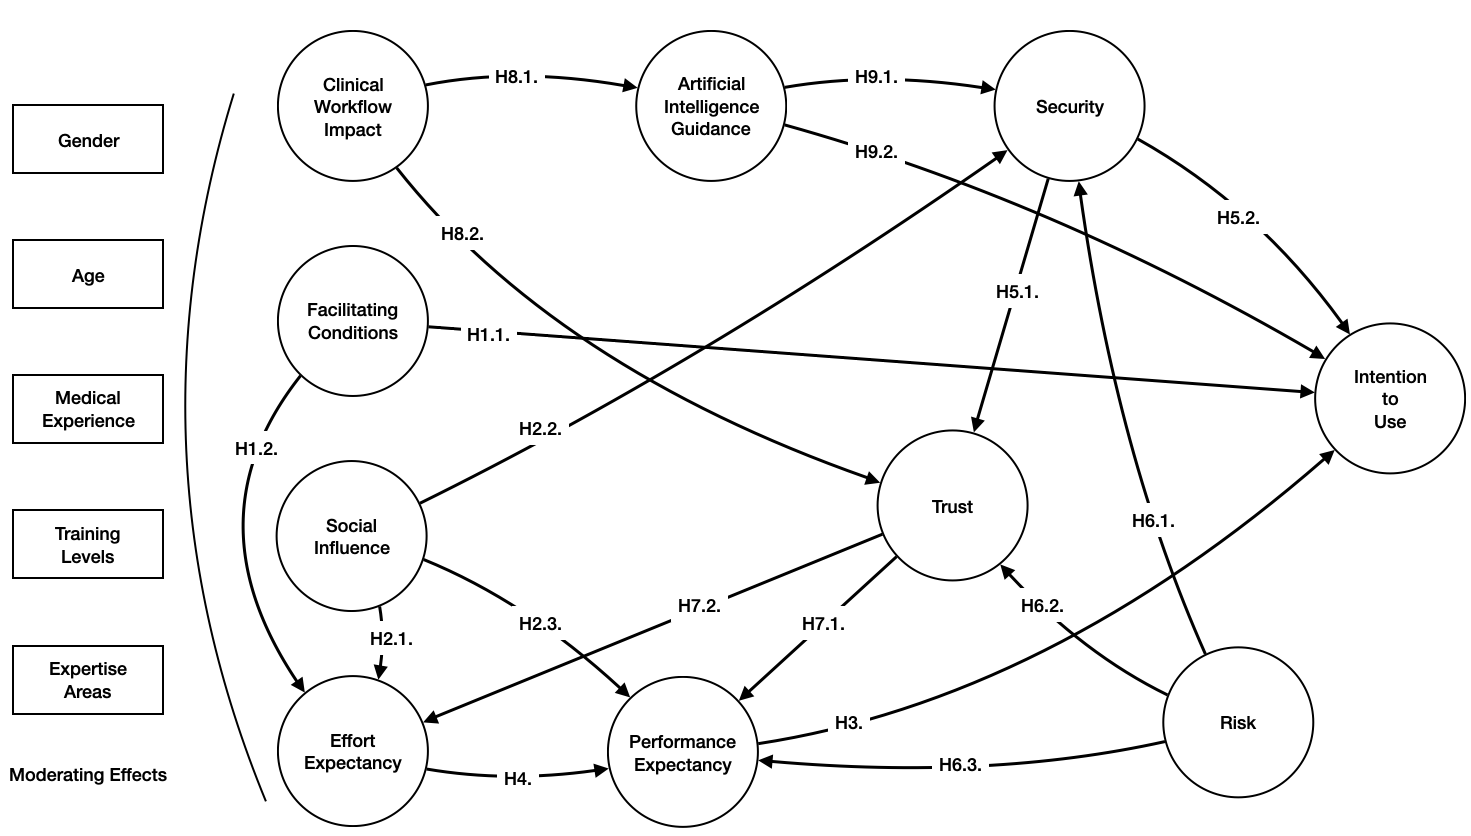
\includegraphics[width=\linewidth]{fig073}
\caption{\textcolor{revised}{The proposed research model, comparing the relations between moderating effects, model constructs, and hypotheses. We adapted this proposed research model from the UTAUT theoretical model to explain the actual adoption of AI in the medical imaging workflow. The research model includes 10 factors. We measured each factor with multiple items. Moreover, we adapted all items from extant literature to improve content validity.}}
\label{fig:fig073}
\end{figure}
%%%%%%%%%%%%%%%%%%%%%%%%%%%%%%%%%%%%%%%%%%%%%%%%%%%

\section{Research Questions \& Hypotheses}
\label{sec:chap004003}

\textcolor{revised}{In this study, we developed a questionnaire grounded in the \ac{UTAUT} model (Figure~\ref{fig:fig073}), which was meticulously adapted to address the unique context of \ac{AI} systems in medical imaging.
This adaptation involved integrating key variables such as trust, perceived usefulness, ease of use, security, risk, and social influence, with a particular emphasis on the nuances of \ac{AI} in the healthcare domain~\cite{BOOTSMAN201999}.
The primary objective was to explore the multifaceted impact of \ac{AI} on technology adoption, delving into aspects such as risk, privacy, and trust, which are critical in the medical imaging context.
Our approach aimed to enhance the questionnaire's explanatory power (Appendix~\ref{chap:app006}), making it more relevant and applicable across diverse \ac{AI} and \ac{HCI} scenarios.}

\textcolor{revised}{To ensure a robust and contextually relevant framework, we formulated hypotheses directly derived from the \ac{UTAUT} constructs, while also integrating insights from contemporary literature on trust, bias, and the explainability of \ac{AI} systems in healthcare~\cite{CHOUDHURY2022103708}.
This approach allowed us to construct a conceptual framework tailored for our exploratory study, focusing specifically on the core determinants of \ac{AI} adoption in medical imaging.
The model was designed to facilitate a nuanced analysis of moderator uncertainties and their potential impacts on these determinants.
The choice of \ac{UTAUT} as our theoretical foundation was informed by its empirical robustness and adaptability, particularly in the context of emerging technologies like \ac{AI} in healthcare settings~\cite{CALISTO2022102922}.
This alignment with the \ac{UTAUT} model, enriched with current literature, ensures that our study not only investigates general adoption patterns but also addresses specific challenges and considerations inherent to \ac{AI}-powered medical imaging systems.}

\subsection{Items Based on UTAUT Constructs}
\label{sec:chap004003001}

Our study takes an exploratory approach to hypothesize the significant effects on user adoption, drawing from the original \ac{UTAUT} constructs.
With these hypotheses, we propose a conceptual framework for our empirical study.
Our model not only covers the core determinants of \ac{AI} adoption, including intention and actual adoption, but also enables the research community to analyze moderator uncertainty that may constrain the effects of these determinants.
Based on its empirical superiority over other models~\cite{CALISTO2022102922}, we choose \ac{UTAUT} as the theoretical foundation for developing our hypotheses.

\vspace{2.00mm}

\noindent
Before describing the hypothesis, let us define {\it behavioral intention} in the context of this thesis:

\vspace{2.00mm}

\textcolor{revised}{{\it Behavioral Intention} is crucial for \ac{AI} tool adoption, reflecting clinicians' willingness to integrate these technologies~\cite{doi:10.1057/ejis.2012.15}.
Influenced by attitudes towards technology, beliefs about \ac{AI}'s efficacy, and the clinical environment, this intention links with trust in the \ac{AI} system, perceptions of biases, and transparency~\cite{Venkatesh2022}.
These factors shape clinicians' readiness to use \ac{AI}, indicating likely usage.
Understanding and influencing this intention bridges theoretical acceptance and practical application, guiding strategies to enhance \ac{AI} acceptance and improve patient care and diagnostic accuracy.}

% \vspace{2.00mm}

\noindent
From here, we specifically developed the following hypotheses:

\vspace{2.00mm}

\textcolor{revised}{{\it Facilitating Conditions} have direct positive relations with user behavior but no effect on behavioral intentions~\cite{CALISTO2022102922}.
Although other authors are using the original \ac{UTAUT} model with separate constructs~\cite{KHALILZADEH2017460}, in this study, we are using behavioral intention as a proxy for user behavior.
In this thesis, it refers to the external factors or circumstances that can either support or hinder a clinician's ability to perform a specific behavior or adopt \ac{AI} technology.}

\vspace{2.00mm}

\noindent
Hence, we hypothesize that:

\vspace{2.00mm}

\noindent
{\bf H1.1.} The facilitating conditions for using \ac{AI} in the clinical workflow, positively predict users' intentions to use it;

\vspace{2.00mm}

\noindent
{\bf H1.2.} The facilitating conditions ({\it e.g.}, ability to use the system) for using \ac{AI} in the clinical workflow, has a direct positive impact on effort expectancy;

\vspace{2.00mm}

{\it Social Influence} has direct impact on behavioral intention.
The underlying assumption is that clinicians tend to consult their medical community about novel diagnosis paradigms and can be influenced by perceived social pressure.
Because perceived security also involves a patient's health for misdiagnosing the case, it should be highly influenced in the proposed model.

\vspace{2.00mm}

\noindent
Based on this, we anticipate that:

\vspace{2.00mm}

\noindent
{\bf H2.1.} The social influence ({\it e.g.}, recommendations from the medical community) for using an \ac{AI} system, positively predicts effort expectancy;

\vspace{2.00mm}

\noindent
{\bf H2.2.} The social influence of using an \ac{AI} system, positively and directly influences perceived security;

\vspace{2.00mm}

\noindent
{\bf H2.3.} The social influence of using an \ac{AI} system, has a direct positive impact on performance expectancy;

\vspace{2.00mm}

{\it Performance Expectancy} is a strong predictor of behavioral intention~\cite{KHALILZADEH2017460}.
It can be divided into utilitarian performance expectancy and hedonic performance expectancy~\cite{CALISTO2022102922}.
While enhancing task performance can increase satisfaction, the effect of hedonic motivation may be weaker, according to some authors~\cite{HART201993}.
In radiology, the ability of \ac{AI} to provide an autonomous second reader that supports decision-making is an attractive goal, offering practical benefits likely to drive adoption.

\vspace{2.00mm}

\noindent
Therefore, we hypothesize that:

\vspace{2.00mm}

\noindent
{\bf H3.} Performance expectancy ({\it i.e.}, usefulness) positively affects behavioral intention to use an \ac{AI} system;

\vspace{2.00mm}

{\it Effort Expectancy} is another predictor of intention to use \ac{AI} systems~\cite{CALISTO2022102922}.
Several authors also find effort expectancy to affect behavioral intention significantly~\cite{KHALILZADEH2017460, HART201993}.
As \ac{AI} provides a new paradigm shift, the perceived degree of ease associated with \ac{AI} systems will likely affect behavioral intention.

% \vspace{2.00mm}

\noindent
In accordance, we denote that:

\vspace{2.00mm}

\noindent
{\bf H4.} Effort expectancy ({\it i.e.}, ease of use) positively affects performance expectancy ({\it i.e.}, usefulness) to use \ac{AI} systems;

% \vspace{2.00mm}

\subsection{Items Based on UTAUT Extensions}
\label{sec:chap004003002}

Trust, security, and risk are pivotal in general technology adoption and play a significant role in sensitive areas like healthcare~\cite{KHALILZADEH2017460}.
The reluctance of clinicians to integrate new technologies in disseminating medical information highlights the need for robust security measures and trust-building strategies to mitigate perceived risks~\cite{10.1145/3132272.3134111}.
This is further emphasized by the increasing concerns about data privacy and the potential misuse of sensitive health information in the digital era~\cite{CALISTO2022102922}.

\vspace{2.00mm}

{\it Perceived Security} is expected to affect behavioral intention directly.
Because \ac{AI} systems involve sensitive patient information, it should be highly influential in the proposed model~\cite{KHALILZADEH2017460}.
Moreover, perceived security is an aggregating construct, changing over time according to medical experts' community opinion and social influence.

\vspace{2.00mm}

\noindent
Therefore, we hypothesize that:

\vspace{2.00mm}

\noindent
{\bf H5.1.} Perceived security of \ac{AI} systems positively and directly predicts perceived trust;

\vspace{2.00mm}

\noindent
{\bf H5.2.} Perceived security of \ac{AI} systems positively and directly behavioral intention to use \ac{AI} systems;

\vspace{2.00mm}

{\it Perceived Risk} is usually related to perceived security.
The more a user perceives the risk, the less secure the user's feel, leading to a negative relationship between risk and security~\cite{KHALILZADEH2017460}.
Indeed, the literature~\cite{10.1145/3132272.3134111, HART201993} states that perceived risk has negative impact on perceived security, and trust, as well as performance expectancy.

\vspace{2.00mm}

\noindent
Based on these literature findings, we formulate the following hypothesis:

\vspace{2.00mm}

\noindent
{\bf H6.1.} The perceived risk of using \ac{AI} systems has a direct negative impact on perceived security;

\vspace{2.00mm}

\noindent
{\bf H6.2.} The perceived risk of using \ac{AI} systems has a direct negative impact on perceived trust;

\vspace{2.00mm}

\noindent
{\bf H6.3.} The perceived risk of using \ac{AI} systems has a direct negative impact on performance expectancy;

\vspace{2.00mm}

{\it Trust} positively affects behavioral intentions~\cite{HART201993}.
As a unitary construct, the effect of trust on behavioral intention has gained notable support.
Moreover, this construct is the most significant predictor of behavioral intention~\cite{CALISTO2022102922, HART201993}.
While \ac{AI}-based solutions become ubiquitous, trust supersedes the importance of traditional adoption factors such as perceived usefulness.
Akin to Khalilzadeh et al.~\cite{KHALILZADEH2017460}, this study includes trust as a singular construct, which is likely to be critical due to the novelty of \ac{AI} systems in the medical workflow and complex environments.

% \vspace{2.00mm}

\noindent
Thus, we hypothesize that:

\vspace{2.00mm}

\noindent
{\bf H7.1.} Trust positively affects performance expectancy ({\it i.e.}, usefulness) to use \ac{AI} systems;

\vspace{2.00mm}

\noindent
{\bf H7.2.} Trust positively affects effort expectancy ({\it i.e.}, ease of use) to use \ac{AI} systems;

% \vspace{2.00mm}

\subsection{Items Related to Impact}
\label{sec:chap004003003}

\ac{AI} has a significant social and personal behavioral impact on the medical community all over the world~\cite{CALISTO2022102922}.
Medical diagnosis impacts significantly on people's health and peoples' lives, and clinicians have to take responsibility for their actions.
Therefore, clinicians may be more cautious than professionals in other fields when considering adopting new technologies to assist their work.
Although clinicians typically resist new technologies, several authors~\cite{doi:10.1148/ryai.2020190043, WAYMEL2019327} are reporting a new behavior change for adopting \ac{AI} systems in the clinical workflow, whereas these systems are increasing clinicians' performance during decision-making \cite{CALISTO2021102607}.

As introduced in Section~\ref{sec:chap004002}, the \ac{TRA} inspires various technology adoption models, arguing that both attitudes toward an action and subjective norms have an impact on behavioral intention, affecting how people perform an action~\cite{CALISTO2022102922}.
Adapted from \ac{TRA} and \ac{TAM}, the \ac{UTAUT} definition of attitude through behavior is ``{\it an individual's positive feeling about performing the target behavior}''~\cite{KHALILZADEH2017460}.
On the other hand, subjective norm refers to ``{\it a person's perception that most people who are important to them think they should or should not perform the behavior in question}''~\cite{WAYMEL2019327}.
\textcolor{revised}{Understanding trust and risk perception is vital for healthcare \ac{AI} integration~\cite{CHOUDHURY2022103708}, with diversity in medical practices and cultural contexts impacting its use in various environments~\cite{Lambert2023}.
Crucial for trust and risk management, diversity in institutional policies and cultural attitudes affects \ac{AI} adoption, effectiveness, and interpretation.}

\vspace{2.00mm}

\noindent
Hence, we hypothesize that:

\vspace{2.00mm}

\noindent
{\bf H8.1.} The extent to which \ac{AI} positively impacts the clinical workflow due to better decision-making of clinicians ({\it e.g.}, decreasing the medical error, time-to-diagnose, etc.), affects the intention to follow \ac{AI} guidance ({\it i.e.}, preferring a timely and less prone to medical error \ac{AI} second-reader);

\vspace{2.00mm}

\noindent
{\bf H8.2.} The extent to which \ac{AI} positively impacts the clinical workflow ({\it e.g.}, decreasing the medical error, time-to-diagnose, etc.) due to better decision-making of clinicians, directly predicts perceived trust;

\vspace{2.00mm}

\textcolor{revised}{Salient beliefs and evaluations shape clinicians' intentions to follow \ac{AI} guidance, but these may not align with factors driving their actual use of \ac{AI}\cite{KHALILZADEH2017460}.
Studies indicate a strong link between trust, perceived risk, and behavioral intentions\cite{GANSSER2021101535, WAYMEL2019327}, yet trust's impact on risk perception does not always translate into actual compliance.
Concerns arise, especially in context-aware applications where \ac{AI} processes subjective data~\cite{10.1145/3313831.3376506}.
This highlights a complex interplay among trust, risk, and compliance in \ac{AI} applications in healthcare settings.}

\textcolor{revised}{Within the \ac{UTAUT} model, our research further explores these dynamics, focusing on what motivates clinicians to follow \ac{AI} guidance in real-world scenarios.
In short, our goal is to investigate how perceived ease of use, performance expectations, and social influence shape clinicians' attitudes towards \ac{AI} adoption.
Additionally, we aim to examine the role of professional experience and specialty in modulating these motivations, recognizing that different medical fields may exhibit varied responses to \ac{AI} integration.
Our study also seeks to understand the threshold at which perceived advantages of \ac{AI} guidance outweigh any reservations, thereby identifying key leverage points for facilitating wider acceptance and effective use of \ac{AI} in medical diagnostics.}

\textcolor{revised}{Existing studies have not explicitly differentiated between factors influencing `intention to follow \ac{AI} guidance' and those affecting clinicians’ actual adherence~\cite{AMEEN2021106548}.
Clinicians may express willingness to adhere to \ac{AI} recommendations, perceiving that the advantages surpass potential risks and security concerns.
However, their actual compliance often hinges on practical factors such as the \ac{AI}'s reliability and organizational policies~\cite{JURAVLE2020263}.
Trust primarily shapes clinicians' willingness and intention, while factors like \ac{AI} performance, security, and institutional norms are more pivotal in their actual decision to follow \ac{AI} guidance.
Therefore, understanding the intricate relationship between trust, intention, and compliance is crucial in designing effective strategies to promote clinicians' acceptance and adherence to \ac{AI} guidance.}

\vspace{2.00mm}

\noindent
Given the wide applicability of \ac{UTAUT}, we can anticipate that:

\vspace{2.00mm}

\noindent
{\bf H9.1.} The willingness to follow the \ac{AI} guidance positively and directly influences perceived security;

\vspace{2.00mm}

\noindent
{\bf H9.2.} The willingness to follow the \ac{AI} guidance positively affects the intention to use AI systems;

% \vspace{2.00mm}

\section{Methods}
\label{sec:chap004004}

Our research model includes ten constructs.
For this study, we measured each construct with multiple items (Figure~\ref{fig:fig075}).
To preserve the content validity and reliability, we measured most of our items from the extant literature~\cite{SOHN2020101324}.
From here, we adjusted these items in our questionnaire to match the context of \ac{AI} adoption among clinicians.
In compliance with recommendations of the two-stage analytical procedure, we used \ac{CFA} to test the measurement model’s validity and reliability~\cite{2019-07124-034}.
In addition, we used \ac{SEM} as a preferable technique to regression.
It allows simultaneous analysis of all relationships through multiple regression, while also allowing for both observed and latent variables to be analyzed simultaneously and providing overall fit statistics.
We conducted \ac{CFA} using the \texttt{R language} (\texttt{v 4.0.2}) employing \ac{MLE}.
Furthermore, \ac{MLE} was then followed by path analysis of the structural relationships conducted in the \texttt{R language} with \ac{SEM} libraries (\texttt{lavaan v. 0.6-7} and \texttt{semTools v. 0.5-3}).
We also undertook moderation analysis in the \texttt{R} language.

%%%%%%%%%%%%%%%%%%%%%%%%%%%%%%%%%%%%%%%%%%%%%%%%%%%
\begin{figure}[htpb]
\centering
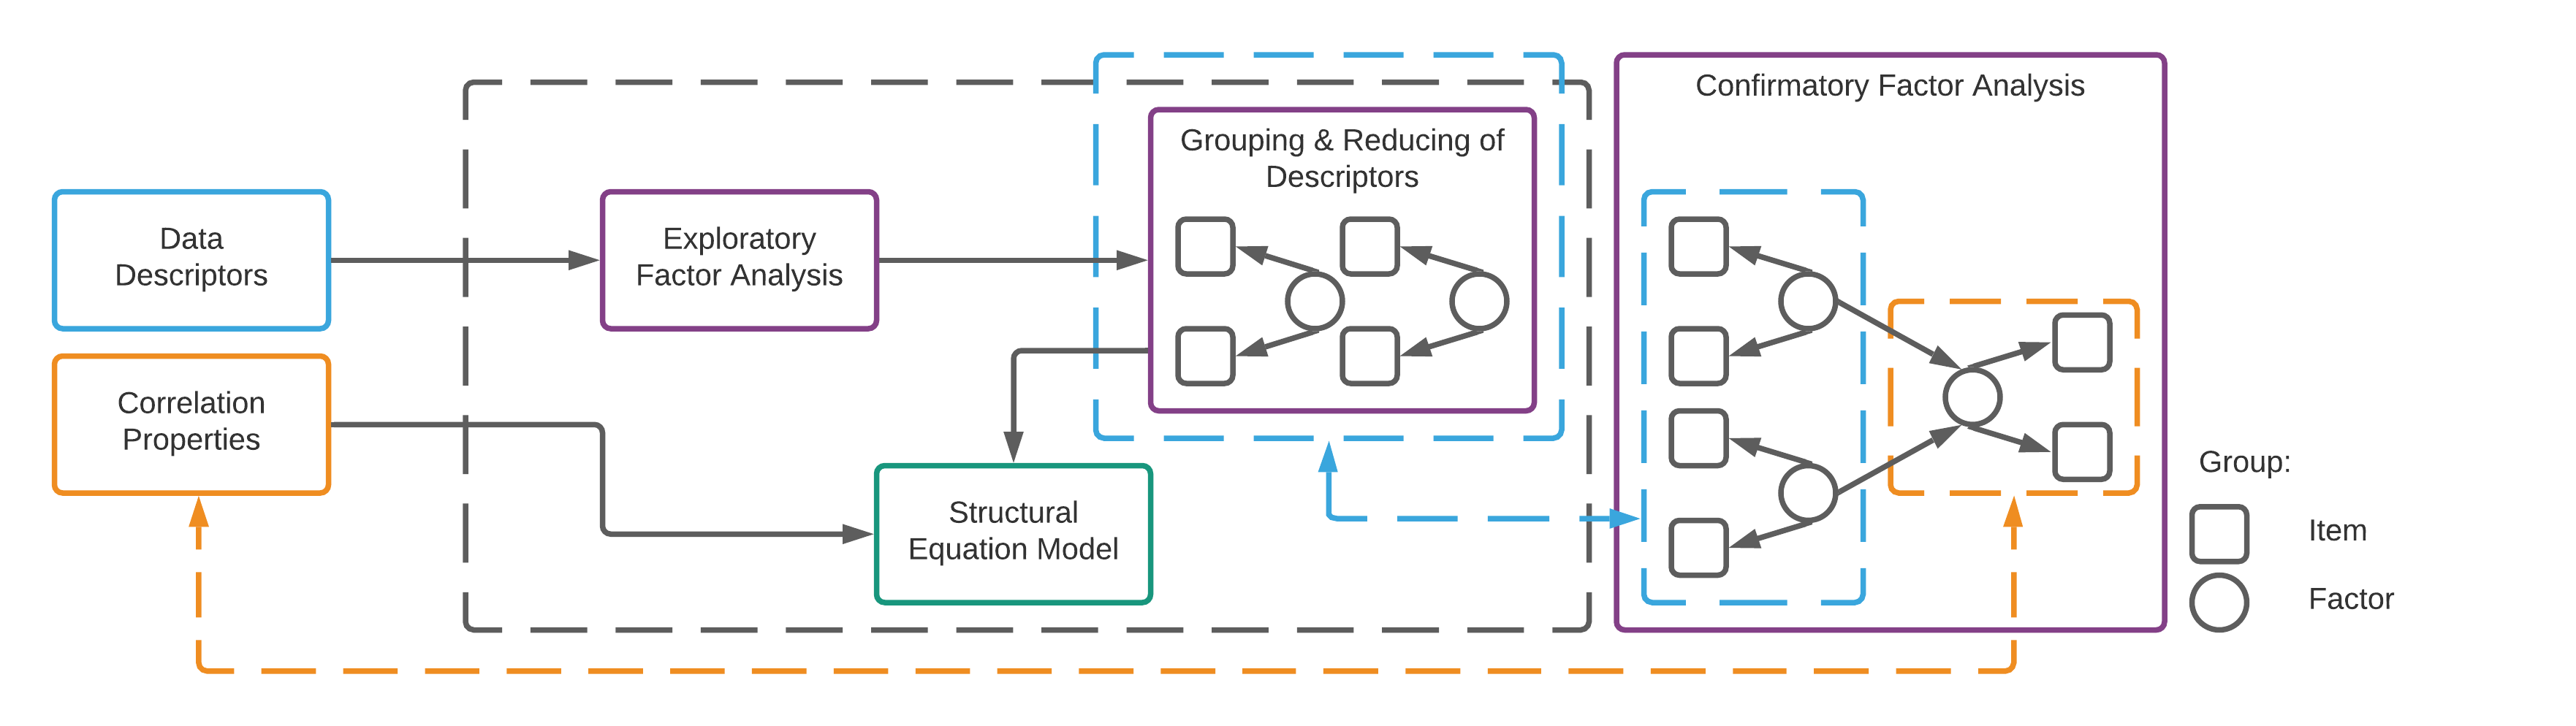
\includegraphics[width=0.985\linewidth]{fig075}
\caption{The basic statistical flow steps followed by us are usually taken in the framework of SEM modeling. Before employing the SEM modeling, we used the conceptual EFA to reduce and group descriptors. Here, we identified the latent factors by using the CFA. Finally, we applied the SEM to estimate the coefficients.}
\label{fig:fig075}
\end{figure}
%%%%%%%%%%%%%%%%%%%%%%%%%%%%%%%%%%%%%%%%%%%%%%%%%%%

\subsection{Procedures}
\label{sec:chap004004001}

We sent the questionnaire via social media ({\it e.g.}, radiology groups on Facebook and LinkedIn) to 17203 participants who gave prior permission to use their data for research purposes under this international study.
The questionnaire contained i) a general explanation of the study, ii) the details of the privacy policy, iii) data treatment, and a iv) link to a Google Forms survey (Appendix~\ref{chap:app006}).
We sent the questionnaire in the middle of February 2021.
The criterion was to send the questionnaire to clinicians worldwide who are members of these social media target groups ({\it i.e.}, radiologists, physicians from any other expertise, technicians, etc.).
Overall, this procedure remained until the end of July 2021, when we analysed and discussed our data.

\subsection{Participants}
\label{sec:chap004004002}

\textcolor{revised}{Table~\ref{tab:tab008}} is listing the sample demographics under this study.
In total, we collected data from 322 participants, corresponding to an overall participation of 1.9\%.
Regarding general demographics (N = 322), the sample consisted of a slightly higher proportion of men (59.9\%) than women (38.8\%) with 1.2\% answering ``Prefer not to say'' during the questionnaire.
For age groups, 12.1\% of participants range from 18 to 29 years old, 29.5\% from 30 to 39, 22.7\% from 40 to 49, 23.9\% from 50 to 59, 10.2\% older than 59, and 1.6 answering ``Prefer not to say'' during the questionnaire.

%%%%%%%%%%%%%%%%%%%%%%%%%%%%%%%%%%%%%%%%%%%%%%%%%%%
\begin{table}[htpb]
\resizebox{\columnwidth}{!}{%
\begin{tabular}{cccc}
\hline
\rule{0mm}{4mm}
Demographic                   & Group                    & Frequency & Percentage
\\
\hline
\multirow[t]{3}{*}{Gender}       & Female                    & 125       & 38.8\%     \\
                                 & Male                      & 193       & 59.9       \\
                                 & Other                     & 4         & 1.2        \\
\hline
\multirow[t]{6}{*}{Age}          & 18 - 29                  & 39        & 12.1\%     \\
                                 & 30 - 39                  & 95        & 29.5\%     \\
                                 & 40 - 49                  & 73        & 22.7\%     \\
                                 & 50 - 59                  & 77        & 23.9\%     \\
                                 & > 59                     & 33        & 10.2\%     \\
                                 & N.A.                     & 5         & 1.6\%      \\
\hline
\multirow[t]{7}{*}{Nationality}  & Europe                   & 126       & 39.2\%     \\
                                 & North America            & 82        & 25.5\%     \\
                                 & Africa                   & 36        & 11.2\%     \\
                                 & Middle East              & 26        & 8.1\%      \\
                                 & Asia                     & 24        & 7.5\%      \\
                                 & Central \& South America & 19        & 5.9\%      \\
                                 & Oceania                  & 9         & 2.8\%      \\
\hline
\multirow[t]{5}{*}{Education}    & Specialists              & 111       & 34.5\%     \\
                                 & Bachelor                 & 81        & 25.2\%     \\
                                 & Master                   & 78        & 24.2\%     \\
                                 & PhD                      & 45        & 14\%       \\
                                 & N.A.                     & 7         & 2.1\%      \\
\hline
\multirow[t]{5}{*}{Medical Experience} & Interns            & 24        & 7.5\%      \\
                                       & Juniors            & 26        & 8.1\%      \\
                                       & Middles            & 54        & 16.5\%     \\
                                       & Seniors            & 210       & 65.2\%     \\
                                       & N.A.               & 8         & 2.4\%      \\
\hline
\multirow[t]{3}{*}{Training Levels}    & Doctors            & 132       & 41\%       \\
                                       & Technicians        & 105       & 32.6\%     \\
                                       & Other              & 85        & 26.4\%     \\
\hline
\end{tabular}%
}
\caption{Characteristics of participants for demographic groups with frequency and percentage. The main characteristics are gender, age, nationality, and education.}
\label{tab:tab008}
\end{table}
%%%%%%%%%%%%%%%%%%%%%%%%%%%%%%%%%%%%%%%%%%%%%%%%%%%

Other demographic data add fundamental insights to this study, such as the medical experience of participants (Section~\ref{chap:app002003001}), training levels (Section~\ref{chap:app002003002}), and expertise areas (Section~\ref{chap:app002003003}).
In this study, the education level of participants is also vital to denote relations between demographic data.
Specifically, 34.5\% of participants are specialists, 25.2\% have at least one bachelor's degree, 24.2\% have a \ac{MSc}, and 14\% have a \ac{PhD} degree.
The other 2.1\% are typically students or academic associate degrees.

\section{Results}
\label{sec:chap004005}

In this study, we examined the sample characteristics of participants (Section~\ref{chap:app002003} of Appendix~\ref{chap:app002}) to gain insights into their profiles and experiences in the medical imaging domain.
\textcolor{revised}{Above, Table~\ref{tab:tab008} presents an overview of these characteristics, shedding light on the typical participant in this study.}
The findings reveal that the typical participant is a radiology specialist in the mid-career stage, primarily working in the public sector.
Most clinicians engage in the analysis of medical imaging exams regularly, with a majority analyzing patients daily.
Furthermore, participants demonstrate varying familiarity with \ac{AI} systems, ranging from awareness without usage to regular utilization.
These insights into the participants' profiles and experiences provide valuable context for understanding their perspectives and behaviors in adopting \ac{AI} technology in healthcare settings.
For a comprehensive summary of all these results, please refer to Section~\ref{chap:app002004006} of Appendix~\ref{chap:app002}.

\subsection{Checking Assumptions}
\label{sec:chap004005001}

The assumptions of the \ac{SEM} were met in this study (Section~\ref{chap:app002004001} of Appendix~\ref{chap:app002}), with normal distributions observed for all variables~\cite{CALISTO2022102922}.
The overall model fit was good~\cite{doi:10.1504/IJMDA.2017.087624}, as indicated by \acp{GFI} of 0.824 surpassing the recommended thresholds.
While some indices were slightly below the recommended levels, the literature suggests that sample size can impact these fit indices~\cite{doi:10.1080/00273171.2019.1602503}.
Notably, the ratio of the test statistic ($\chi^2$) to the degree of freedom ($df$) was within the recommended range ($\chi^2$ / $df$ = 2.587 $<$ 3.0), and both \ac{RMSEA} and \ac{SRMR} of 0.083 indicated an acceptable model fit~\cite{ZHOU2010760}.
Despite a significant $\chi^2$ value due to the large sample size, the Hoelter index confirmed that the sample adequately supported the sophisticated model~\cite{CALISTO2022102922}.

\subsection{Measurement Model}
\label{sec:chap004005002}

Convergent and discriminant validity were examined to ensure the robustness of the measurement model~\cite{CALISTO2022102922}.
All item loadings were significant (p-value = 0.000), indicating good convergent validity, with most loadings above 0.8~\cite{CALISTO2022102922}.
Each item significantly loaded on its respective construct, demonstrating convergent validity.
Discriminant validity was confirmed by comparing shared variance and \ac{AVE}, with shared variance lower than \ac{AVE}.
The measurement model exhibited good reliability, with a \ac{CR} of 0.95~\cite{doi:10.1504/IJMDA.2017.087624}.
These findings confirm the reliability, convergent validity, and discriminant validity of the measurement model.
Moderating effects on other variables (Section~\ref{sec:chap004005005}), particularly demographics, warrant further investigation.
\textcolor{revised}{Comprehensive findings from the \ac{CFA} are detailed in Table~\ref{tab:tab009}.
For an in-depth analysis, additional information and expanded results of the \ac{CFA} can be found in Section~\ref{chap:app002004002} of Appendix~\ref{chap:app002}.}

%%%%%%%%%%%%%%%%%%%%%%%%%%%%%%%%%%%%%%%%%%%%%%%%%%%
\begin{table*}
\resizebox{\textwidth}{!}{%
\begin{tabular}{ccccccccccc}
\hline
Measure & Impact & Guidance & PerfExp & EffExp & SocInf & FacCond & IntUse & Security & Risk & Trust \\ \hline
alpha   & 0.57   & 0.88     & 0.87    & 0.89   & 0.73   & 0.80    & 0.94   & 0.83     & 0.84    & 0.88  \\
CR      & 0.57   & 0.88     & 0.89    & 0.89   & 0.74   & 0.79    & 0.93   & 0.82     & 0.84    & 0.88  \\
AVE     & 0.40   & 0.65     & 0.72    & 0.73   & 0.49   & 0.55    & 0.78   & 0.60     & 0.64    & 0.70  \\ \hline
\end{tabular}%
}
\caption{The abbreviated constructs are as follows: Clinical Workflow Impact (Impact); AI Guidance (Guidance); Performance Expectancy (PerfExp); Effort Expectancy (EffExp); Social Influence (SocInf); Facilitating Conditions (FacCond); Behavior Intention to Use (IntUse); Perceived Security (Security); Perceived Risk (Risk); Perceived Trust (Trust). Moreover, the measure abbreviations are: Cronbach alpha (alpha); Composite Reliability (CR); Average Variance Extracted (AVE).}
\label{tab:tab009}
\end{table*}
%%%%%%%%%%%%%%%%%%%%%%%%%%%%%%%%%%%%%%%%%%%%%%%%%%%

\subsection{Parallel Analysis}
\label{sec:chap004005003}

Parallel analysis was conducted to determine the appropriate number of factors to retain in the measurement model~\cite{doi:10.1080/10705511.2019.1615835}.
By simulating eigenvalues based on the number of items and sample size, the parallel analysis compares these simulated eigenvalues with the eigenvalues obtained from the study \textcolor{revised}{(Figure~\ref{fig:fig093})}.
Factors with eigenvalues that overlap with the cutoff line for retention indicate potential factors to consider.
The scree plot in \textcolor{revised}{Figure~\ref{fig:fig093}} shows notable changes in effect size, suggesting a breakpoint for the number of factors.
However, the decision to retain factors is not solely based on these changes; it also considers the line limits of the parallel analysis.

%%%%%%%%%%%%%%%%%%%%%%%%%%%%%%%%%%%%%%%%%%%%%%%%%%%
\begin{figure}[htpb]
\centering
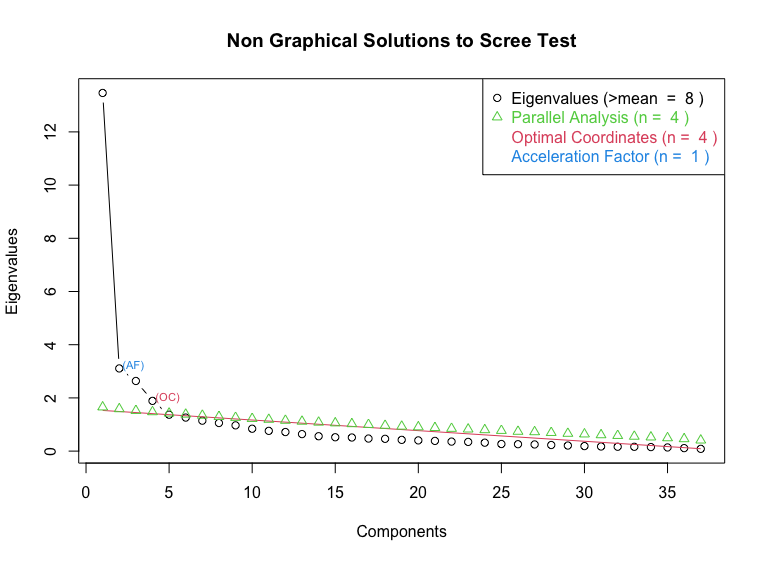
\includegraphics[width=0.955\linewidth]{fig093}
\caption{\textcolor{revised}{Scree plot of eigenvalues with the eigenvalues greater than one rule, elbow bend, and intersecting lines.}}
\label{fig:fig093}
\end{figure}
%%%%%%%%%%%%%%%%%%%%%%%%%%%%%%%%%%%%%%%%%%%%%%%%%%%

The difference in eigenvalues becomes more significant when comparing the fifth and sixth components, as well as the sixth and seventh components.
Components eight and nine are mainly below the line, highlighting the arbitrary nature of item retention for factors or overall models~\cite{CALISTO2022102922}.
Therefore, the analysis suggests retaining factors up to the seventh component, resulting in a total of seven factors in the measurement model.
More details on the parallel analysis results will be described in Section~\ref{chap:app002004003} of Appendix~\ref{chap:app002}.

\subsection{Structural Model}
\label{sec:chap004005004}

The satisfactory fit of the measurement model allowed us to employ \ac{SEM} for data analysis.
\ac{SEM} evaluates the extent to which the collected data align with the theoretical model's measurement~\cite{doi:10.1080/10705511.2017.1401932}.
In this study, we extended the proposed research model by introducing two new constructs:
(1) Clinical Workflow Impact; and
(2) \ac{AI} Guidance.
These additions enabled us to explore the interactions between these constructs and existing variables within the model.
We assessed the structural relationships by estimating the hypothesized causal paths, with the majority of hypotheses supported (except for {\bf H6.1}, {\bf H6.3}, and {\bf H7.1}) based on a significance level of {\it p-value} $<$ 0.10 from \textcolor{revised}{Table~\ref{tab:tab011}}.
For a more comprehensive analysis of \ac{SEM} and its evaluation, refer to Section~\ref{chap:app002004004} of Appendix~\ref{chap:app002}.
This section provides detailed insights into the relationships between variables \textcolor{revised}{(Table~\ref{tab:tab010})}, further supporting our findings.

%%%%%%%%%%%%%%%%%%%%%%%%%%%%%%%%%%%%%%%%%%%%%%%%%%%
\begin{table}[htpb]
\resizebox{\columnwidth}{!}{%
\begin{tabular}{lrrrrrl}
\hline
Hypotheses & \multicolumn{1}{l}{b} & \multicolumn{1}{l}{StdError} & \multicolumn{1}{l}{z-value} & \multicolumn{1}{l}{p-value} & \multicolumn{1}{l}{beta} & Supported \\
\hline
\textbf{H1.1.} & 0.313  & 0.053 & 5.912  & 0.000 & 0.349  & Yes ***                  \\
\textbf{H1.2.} & 0.432  & 0.08  & 5.393  & 0.000 & 0.375  & Yes ***                  \\
\textbf{H2.1.} & 0.268  & 0.133 & 2.015  & 0.044 & 0.211  & Yes **                   \\
\textbf{H2.2.} & 0.432  & 0.08  & 5.393  & 0.000 & 0.375  & Yes ***                  \\
\textbf{H2.3}  & 0.239  & 0.067 & 3.554  & 0.000 & 0.243  & Yes ***                  \\
\textbf{H3.}   & 0.327  & 0.068 & 4.81   & 0.000 & 0.264  & Yes ***                  \\
\textbf{H4.}   & 0.466  & 0.061 & 7.653  & 0.000 & 0.603  & Yes ***                  \\
\textbf{H5.1.} & 0.701  & 0.078 & 9.012  & 0.000 & 0.715  & Yes ***                  \\
\textbf{H5.2.} & 0.239  & 0.06  & 4.005  & 0.000 & 0.226  & Yes ***                  \\
\textbf{H6.1.} & -0.016 & 0.049 & -0.326 & 0.744 & -0.02  & \textcolor{red}{No}      \\
\textbf{H6.2.} & -0.098 & 0.059 & -1.672 & 0.095 & -0.124 & Yes *                    \\
\textbf{H6.3.} & -0.031 & 0.033 & -0.962 & 0.336 & -0.046 & \textcolor{red}{No}      \\
\textbf{H7.1.} & 0.009  & 0.045 & 0.197  & 0.844 & 0.01   & \textcolor{red}{No}      \\
\textbf{H7.2.} & 0.375  & 0.062 & 6.014  & 0.000 & 0.333  & Yes ***                  \\
\textbf{H8.1.} & -0.494 & 0.09  & -5.512 & 0.000 & -0.487 & Yes ***                  \\
\textbf{H8.2.} & 0.176  & 0.092 & 1.92   & 0.055 & 0.179  & Yes *                    \\
\textbf{H9.1.} & 0.459  & 0.067 & 6.861  & 0.000 & 0.464  & Yes ***                  \\
\textbf{H9.2.} & 0.336  & 0.055 & 6.151  & 0.000 & 0.322  & Yes ***                  \\
\hline
\end{tabular}%
}
\caption{Summary of hypothesis tests. The variables assigned to the significance values are as follows: *** significant at level $\alpha = 0.01$; ** significant at level $\alpha = 0.05$; and * significant fixed at level $\alpha = 0.10$.}
\label{tab:tab011}
\end{table}
%%%%%%%%%%%%%%%%%%%%%%%%%%%%%%%%%%%%%%%%%%%%%%%%%%%

\clearpage

%%%%%%%%%%%%%%%%%%%%%%%%%%%%%%%%%%%%%%%%%%%%%%%%%%%
\begin{table}[htpb]
\resizebox{\columnwidth}{!}{%
\begin{tabular}{llrrrl}
\hline
Construct                   & Item        & \multicolumn{1}{l}{Alpha} & \multicolumn{1}{l}{StdError} & \multicolumn{1}{l}{z-value} & p-value \\ \hline
Clinical Workflow Impact & Impact\_1   & 0.53 & 0.080 & 6.615  & 0.000 \\
Alpha = 0.57                & Impact\_2   & 0.75  & 0.079    & 9.499   & 0.000   \\ \hline
AI Guidance              & Guidance\_1 & 0.36 & 0.035 & 10.209 & 0.000 \\
Alpha = 0.88             & Guidance\_2 & 0.29 & 0.028 & 10.102 & 0.000 \\
R2 = 0.238                  & Guidance\_3 & 0.19  & 0.026    & 7.262   & 0.000   \\
                            & Guidance\_4 & 0.32  & 0.033    & 9.683   & 0.000   \\ \hline
Performance Expectancy      & PerfExp\_1  & 0.45                      & 0.039                        & 11.606                      & 0.000   \\
Alpha = 0.87                & PerfExp\_2  & 0.14                      & 0.019                        & 7.186                       & 0.000   \\
R2 = 0.595                  & PerfExp\_3  & 0.08                      & 0.018                        & 4.382                       & 0.000   \\ \hline
Effort Expectancy           & EffExp\_1   & 0.16                      & 0.022                        & 7.335                       & 0.000   \\
Alpha = 0.89                & EffExp\_2   & 0.19                      & 0.021                        & 8.615                       & 0.000   \\
R2 = 0.496                  & EffExp\_3   & 0.25                      & 0.025                        & 9.821                       & 0.000   \\ \hline
Social Influence            & SocInf\_1   & 0.57                      & 0.054                        & 10.464                      & 0.000   \\
Alpha = 0.73                & SocInf\_2   & 0.68                      & 0.066                        & 10.24                       & 0.000   \\
                            & SocInf\_3   & 0.35                      & 0.047                        & 7.356                       & 0.000   \\ \hline
Facilitating Conditions     & FacCond\_1  & 0.56                      & 0.06                         & 9.284                       & 0.000   \\
Alpha = 0.80                & FacCond\_2  & 0.57                      & 0.061                        & 9.45                        & 0.000   \\
                            & FacCond\_3  & 0.41                      & 0.046                        & 8.932                       & 0.000   \\ \hline
Behavioral Intention to Use & IntUse\_1   & 0.16                      & 0.017                        & 9.576                       & 0.000   \\
Alpha = 0.94                & IntUse\_2   & 0.13                      & 0.015                        & 8.496                       & 0.000   \\
R2 = 0.681                  & IntUse\_3   & 0.15                      & 0.016                        & 9.761                       & 0.000   \\
                            & IntUse\_4   & 0.19                      & 0.019                        & 9.856                       & 0.000   \\ \hline
Security                    & Security\_1 & 0.41                      & 0.041                        & 10.055                      & 0.000   \\
Alpha = 0.83                & Security\_2 & 0.14                      & 0.025                        & 5.621                       & 0.000   \\
R2 = 0.397                  & Security\_3 & 0.39                      & 0.037                        & 10.537                      & 0.000   \\ \hline
Risk                        & Risk\_1  & 0.36                         & 0.049                        & 7.342                       & 0.000   \\
Alpha = 0.84                & Risk\_2  & 0.57                         & 0.06                         & 9.48                        & 0.000   \\
                            & Risk\_3  & 0.34                         & 0.047                        & 7.114                       & 0.000   \\ \hline
Trust                       & Trust\_1    & 0.30                      & 0.031                        & 9.762                       & 0.000   \\
Alpha = 0.88                & Trust\_2    & 0.19                      & 0.025                        & 7.606                       & 0.000   \\
R2 = 0.465                  & Trust\_3    & 0.21                      & 0.029                        & 7.385                       & 0.000  \\ \hline
\end{tabular}%
}
\caption{The measuring model with: Clinical Workflow Impact ({\bf Impact}); AI Guidance ({\bf Guidance}); Performance Expectancy ({\bf PerfExp}); Effort Expectancy ({\bf EffExp}); Social Influence ({\bf SocInf}); Facilitating Conditions ({\bf FacCond}); Behavioral Intention to Use ({\bf IntUse}); {\bf Security}; {\bf Risk}; and {\bf Trust}. The computed measurements are {\bf Alpha}, Standard Error ({\bf StdError}), {\bf z-value}, and {\bf p-value}.}
\label{tab:tab010}
\end{table}
%%%%%%%%%%%%%%%%%%%%%%%%%%%%%%%%%%%%%%%%%%%%%%%%%%%

\clearpage

The coefficient of determination ($R^2$), also known as \ac{SMC}, provides insights into the explanatory power and predictive accuracy of the measurement model \textcolor{revised}{(Table~\ref{tab:tab010})}.
Higher loadings indicate stronger relationships between the items and their corresponding latent constructs.
\textcolor{revised}{In the context of the \ac{UTAUT} model, a high $R^2$ value indicates an effective capture of variance in user acceptance and technology usage behavior.
This is vital for validating the model's robustness and assessing the impact of its constructs on technology adoption.}

Behavioral intention exhibited the highest value ($R^2$ = 0.681), indicating a substantial amount of variance explained.
Conversely, \ac{AI} Guidance had the lowest value ($R^2$ = 0.238), followed by security ($R^2$ = 0.397).
These lower values can be attributed to their close association with independent variables and the inherent nature of the constructs, which are influenced by a clinician's belief in \ac{AI} systems.
The coefficient for performance expectancy ($R^2$ = 0.595), effort expectancy ($R^2$ = 0.496), and trust ($R^2$ = 0.465) were also acceptable, which is consistent with previous results~\cite{KHALILZADEH2017460}.
These coefficients indicate the extent to which the independent variables can account for the variance in the dependent variable.

\subsection{Moderating Effects}
\label{sec:chap004005005}

To examine potential moderator effects, we conducted a comprehensive analysis using the split sample approach \cite{LI2021106581, LI2021106929}.
We investigated the moderation of gender, age, nationality, education, and clinical knowledge on the relationships within our research model.
Notably, significant moderating effects were found for all variables, providing insights into the nuanced dynamics and contextual influences within the model.
The detailed results are presented in Table~\ref{tab:tab012}, which includes the path coefficients and significance levels for each moderator variable.
These findings underscore the importance of considering demographic factors in understanding the relationships in our study.

%%%%%%%%%%%%%%%%%%%%%%%%%%%%%%%%%%%%%%%%%%%%%%%%%%%
\begin{table}[htpb]
\resizebox{\textwidth}{!}{%
\begin{tabular}{|l|ll|ll|ll|ll|ll|}
\hline
\multicolumn{1}{|c|}{\multirow{2}{*}{Hypotheses}} &
  \multicolumn{2}{c|}{Gender} &
  \multicolumn{2}{c|}{Age} &
  \multicolumn{2}{c|}{Nationality Classification} &
  \multicolumn{2}{c|}{Education} &
  \multicolumn{2}{c|}{Knowledge} \\ \cline{2-11} 
\multicolumn{1}{|c|}{} &
  \multicolumn{1}{c|}{Woman} &
  \multicolumn{1}{c|}{Man} &
  \multicolumn{1}{c|}{\textless 30} &
  \multicolumn{1}{c|}{\textgreater{}= 30} &
  \multicolumn{1}{c|}{Developed} &
  \multicolumn{1}{c|}{Developing} &
  \multicolumn{1}{c|}{Higher} &
  \multicolumn{1}{c|}{Advanced} &
  \multicolumn{1}{c|}{Expert} &
  \multicolumn{1}{c|}{Novice} \\ \hline
\textbf{H1.1.} &
  \multicolumn{1}{l|}{$\textcolor{red}{\downarrow}$ 0.39 ***} &
  $\textcolor{blue}{\uparrow}$ 0.64 *** &
  \multicolumn{1}{l|}{$\textcolor{red}{\downarrow}$ 0.09 \textcolor{red}{ns}} &
  0.57 *** &
  \multicolumn{1}{l|}{$\textcolor{red}{\downarrow}$ 0.59 ***} &
  $\textcolor{red}{\downarrow}$ 0.36 *** &
  \multicolumn{1}{l|}{0.53 ***} &
  $\textcolor{red}{\downarrow}$ 0.33 *** &
  \multicolumn{1}{l|}{0.59 ***} &
  $\textcolor{red}{\downarrow}$ 0.23 ** \\ \hline
\textbf{H1.2.} &
  \multicolumn{1}{l|}{$\textcolor{red}{\downarrow}$ 0.36 ***} &
  $\textcolor{blue}{\uparrow}$ 0.61 *** &
  \multicolumn{1}{l|}{$\textcolor{red}{\downarrow}$ 0.09 \textcolor{red}{ns}} &
  $\textcolor{blue}{\uparrow}$ 0.59 *** &
  \multicolumn{1}{l|}{$\textcolor{red}{\downarrow}$ 0.47 ***} &
  $\textcolor{red}{\downarrow}$ 0.33 *** &
  \multicolumn{1}{l|}{0.51 ***} &
  $\textcolor{red}{\downarrow}$ 0.26 *** &
  \multicolumn{1}{l|}{$\textcolor{blue}{\uparrow}$ 0.59 ***} &
  $\textcolor{red}{\downarrow}$ 0.12 \textcolor{red}{ns} \\ \hline
\textbf{H2.1.} &
  \multicolumn{1}{l|}{$\textcolor{blue}{\uparrow}$ 0.38 ***} &
  $\textcolor{blue}{\uparrow}$ 0.54 *** &
  \multicolumn{1}{l|}{$\textcolor{red}{\downarrow}$ 0.11 \textcolor{red}{ns}} &
  $\textcolor{blue}{\uparrow}$ 0.56 *** &
  \multicolumn{1}{l|}{$\textcolor{blue}{\uparrow}$ 0.39 ***} &
  $\textcolor{blue}{\uparrow}$ 0.41 *** &
  \multicolumn{1}{l|}{$\textcolor{blue}{\uparrow}$ 0.47 ***} &
  $\textcolor{blue}{\uparrow}$ 0.35 *** &
  \multicolumn{1}{l|}{$\textcolor{blue}{\uparrow}$ 0.56 ***} &
  $\textcolor{red}{\downarrow}$ 0.15 \textcolor{red}{ns} \\ \hline
\textbf{H2.2.} &
  \multicolumn{1}{l|}{$\textcolor{red}{\downarrow}$ 0.27 **} &
  0.54 *** &
  \multicolumn{1}{l|}{$\textcolor{red}{\downarrow}$ 0.11 \textcolor{red}{ns}} &
  0.56 *** &
  \multicolumn{1}{l|}{$\textcolor{red}{\downarrow}$ 0.35 ***} &
  $\textcolor{red}{\downarrow}$ 0.36 *** &
  \multicolumn{1}{l|}{0.47 ***} &
  $\textcolor{red}{\downarrow}$ 0.24 ** &
  \multicolumn{1}{l|}{0.49 ***} &
  $\textcolor{red}{\downarrow}$ 0.15 \textcolor{red}{ns} \\ \hline
\textbf{H2.3} &
  \multicolumn{1}{l|}{0.36 ***} &
  $\textcolor{blue}{\uparrow}$ 0.51 *** &
  \multicolumn{1}{l|}{$\textcolor{red}{\downarrow}$ 0.18 *} &
  $\textcolor{blue}{\uparrow}$ 0.54 *** &
  \multicolumn{1}{l|}{$\textcolor{blue}{\uparrow}$ 0.55 ***} &
  0.38 *** &
  \multicolumn{1}{l|}{$\textcolor{blue}{\uparrow}$ 0.48 ***} &
  0.34 *** &
  \multicolumn{1}{l|}{$\textcolor{blue}{\uparrow}$ 0.52 ***} &
  $\textcolor{red}{\downarrow}$ 0.18 * \\ \hline
\textbf{H3.} &
  \multicolumn{1}{l|}{0.46 ***} &
  $\textcolor{blue}{\uparrow}$ 0.63 *** &
  \multicolumn{1}{l|}{$\textcolor{red}{\downarrow}$ 0.24 ***} &
  $\textcolor{blue}{\uparrow}$ 0.66 *** &
  \multicolumn{1}{l|}{0.55 ***} &
  0.47 *** &
  \multicolumn{1}{l|}{0.58 ***} &
  0.42 *** &
  \multicolumn{1}{l|}{$\textcolor{blue}{\uparrow}$ 0.68 ***} &
  $\textcolor{red}{\downarrow}$ 0.26 *** \\ \hline
\textbf{H4.} &
  \multicolumn{1}{l|}{$\textcolor{red}{\downarrow}$ 0.47 ***} &
  0.67 *** &
  \multicolumn{1}{l|}{$\textcolor{red}{\downarrow}$ 0.33 ***} &
  0.63 *** &
  \multicolumn{1}{l|}{$\textcolor{red}{\downarrow}$ 0.51 ***} &
  $\textcolor{red}{\downarrow}$ 0.46 *** &
  \multicolumn{1}{l|}{0.58 ***} &
  $\textcolor{red}{\downarrow}$ 0.38 *** &
  \multicolumn{1}{l|}{0.67 ***} &
  $\textcolor{red}{\downarrow}$ 0.27 *** \\ \hline
\textbf{H5.1.} &
  \multicolumn{1}{l|}{$\textcolor{red}{\downarrow}$ 0.33 ***} &
  0.65 *** &
  \multicolumn{1}{l|}{$\textcolor{red}{\downarrow}$ 0.34 ***} &
  0.58 *** &
  \multicolumn{1}{l|}{$\textcolor{red}{\downarrow}$ 0.45 ***} &
  $\textcolor{red}{\downarrow}$ 0.44 *** &
  \multicolumn{1}{l|}{0.59 ***} &
  $\textcolor{red}{\downarrow}$ 0.27 *** &
  \multicolumn{1}{l|}{0.58 ***} &
  $\textcolor{red}{\downarrow}$ 0.34 *** \\ \hline
\textbf{H5.2.} &
  \multicolumn{1}{l|}{0.42 ***} &
  $\textcolor{blue}{\uparrow}$ 0.66 *** &
  \multicolumn{1}{l|}{$\textcolor{red}{\downarrow}$ 0.14 \textcolor{red}{ns}} &
  $\textcolor{blue}{\uparrow}$ 0.68 *** &
  \multicolumn{1}{l|}{$\textcolor{blue}{\uparrow}$ 0.68 ***} &
  0.35 *** &
  \multicolumn{1}{l|}{$\textcolor{blue}{\uparrow}$ 0.57 ***} &
  0.38 *** &
  \multicolumn{1}{l|}{$\textcolor{blue}{\uparrow}$ 0.64 ***} &
  $\textcolor{red}{\downarrow}$ 0.19 ** \\ \hline
\textbf{H6.1.} &
  \multicolumn{1}{l|}{$\textcolor{blue}{\uparrow}$ -0.21 **} &
  $\textcolor{blue}{\uparrow}$ 0.17 * &
  \multicolumn{1}{l|}{$\textcolor{blue}{\uparrow}$ 0.11 \textcolor{red}{ns}} &
  -0.04 \textcolor{red}{ns} &
  \multicolumn{1}{l|}{$\textcolor{red}{\downarrow}$ -0.16 *} &
  $\textcolor{blue}{\uparrow}$ 0.17 * &
  \multicolumn{1}{l|}{0.08 \textcolor{red}{ns}} &
  $\textcolor{red}{\downarrow}$ -0.15 \textcolor{red}{ns} &
  \multicolumn{1}{l|}{-0.02 \textcolor{red}{ns}} &
  0.86 \textcolor{red}{ns} \\ \hline
\textbf{H6.2.} &
  \multicolumn{1}{l|}{-0.21 **} &
  0.13 \textcolor{red}{ns} &
  \multicolumn{1}{l|}{$\textcolor{red}{\downarrow}$ 0.01 \textcolor{red}{ns}} &
  $\textcolor{red}{\downarrow}$ -0.06 \textcolor{red}{ns} &
  \multicolumn{1}{l|}{$\textcolor{red}{\downarrow}$ -0.13 \textcolor{red}{ns}} &
  $\textcolor{red}{\downarrow}$ 0.02 \textcolor{red}{ns} &
  \multicolumn{1}{l|}{$\textcolor{red}{\downarrow}$ 0.01 \textcolor{red}{ns}} &
  $\textcolor{red}{\downarrow}$ -0.12 \textcolor{red}{ns} &
  \multicolumn{1}{l|}{$\textcolor{red}{\downarrow}$ -0.04 \textcolor{red}{ns}} &
  $\textcolor{red}{\downarrow}$ -0.03 \textcolor{red}{ns} \\ \hline
\textbf{H6.3.} &
  \multicolumn{1}{l|}{$\textcolor{red}{\downarrow}$ -0.22 **} &
  $\textcolor{blue}{\uparrow}$ 0.09 \textcolor{red}{ns} &
  \multicolumn{1}{l|}{0.04 \textcolor{red}{ns}} &
  -0.13 \textcolor{red}{ns} &
  \multicolumn{1}{l|}{$\textcolor{red}{\downarrow}$ -0.18 *} &
  -0.01 \textcolor{red}{ns} &
  \multicolumn{1}{l|}{-0.11 \textcolor{red}{ns}} &
  -0.07 \textcolor{red}{ns} &
  \multicolumn{1}{l|}{$\textcolor{red}{\downarrow}$ -0.18 *} &
  $\textcolor{blue}{\uparrow}$ 0.13 \textcolor{red}{ns} \\ \hline
\textbf{H7.1.} &
  \multicolumn{1}{l|}{0.12 \textcolor{red}{ns}} &
  $\textcolor{blue}{\uparrow}$ 0.53 *** &
  \multicolumn{1}{l|}{0.17 *} &
  $\textcolor{blue}{\uparrow}$ 0.44 *** &
  \multicolumn{1}{l|}{$\textcolor{blue}{\uparrow}$ 0.28 **} &
  $\textcolor{blue}{\uparrow}$ 0.37 *** &
  \multicolumn{1}{l|}{$\textcolor{blue}{\uparrow}$ 0.39 ***} &
  $\textcolor{blue}{\uparrow}$ 0.24 ** &
  \multicolumn{1}{l|}{$\textcolor{blue}{\uparrow}$ 0.46 ***} &
  0.11 \textcolor{red}{ns} \\ \hline
\textbf{H7.2.} &
  \multicolumn{1}{l|}{$\textcolor{red}{\downarrow}$ 0.23 **} &
  0.63 *** &
  \multicolumn{1}{l|}{$\textcolor{red}{\downarrow}$ 0.15 \textcolor{red}{ns}} &
  0.53 *** &
  \multicolumn{1}{l|}{$\textcolor{red}{\downarrow}$ 0.36 ***} &
  $\textcolor{red}{\downarrow}$ 0.39 *** &
  \multicolumn{1}{l|}{$\textcolor{red}{\downarrow}$ 0.46 ***} &
  $\textcolor{red}{\downarrow}$ 0.29 *** &
  \multicolumn{1}{l|}{0.55 ***} &
  $\textcolor{red}{\downarrow}$0.06 \textcolor{red}{ns} \\ \hline
\textbf{H8.1.} &
  \multicolumn{1}{l|}{$\textcolor{blue}{\uparrow}$ -0.25 **} &
  $\textcolor{blue}{\uparrow}$ -0.42 *** &
  \multicolumn{1}{l|}{$\textcolor{blue}{\uparrow}$ -0.23 **} &
  -0.50 *** &
  \multicolumn{1}{l|}{-0.49 ***} &
  $\textcolor{blue}{\uparrow}$ -0.22 ** &
  \multicolumn{1}{l|}{$\textcolor{blue}{\uparrow}$ -0.34 ***} &
  $\textcolor{blue}{\uparrow}$ -0.41 *** &
  \multicolumn{1}{l|}{-0.53 ***} &
  $\textcolor{blue}{\uparrow}$ -0.09 \textcolor{red}{ns} \\ \hline
\textbf{H8.2.} &
  \multicolumn{1}{l|}{$\textcolor{red}{\downarrow}$ -0.09 \textcolor{red}{ns}} &
  -0.11 \textcolor{red}{ns} &
  \multicolumn{1}{l|}{0.11 \textcolor{red}{ns}} &
  -0.21 ** &
  \multicolumn{1}{l|}{-0.14 \textcolor{red}{ns}} &
  -0.14 \textcolor{red}{ns} &
  \multicolumn{1}{l|}{$\textcolor{blue}{\uparrow}$ -0.09 \textcolor{red}{ns}} &
  -0.12 \textcolor{red}{ns} &
  \multicolumn{1}{l|}{-0.21 **} &
  $\textcolor{blue}{\uparrow}$ 0.07 \textcolor{red}{ns} \\ \hline
\textbf{H9.1.} &
  \multicolumn{1}{l|}{$\textcolor{red}{\downarrow}$ 0.39 ***} &
  0.58 *** &
  \multicolumn{1}{l|}{$\textcolor{red}{\downarrow}$ 0.32 ***} &
  0.55 *** &
  \multicolumn{1}{l|}{$\textcolor{red}{\downarrow}$ 0.39 ***} &
  $\textcolor{red}{\downarrow}$ 0.38 *** &
  \multicolumn{1}{l|}{$\textcolor{red}{\downarrow}$ 0.44 ***} &
  $\textcolor{red}{\downarrow}$ 0.34 *** &
  \multicolumn{1}{l|}{$\textcolor{red}{\downarrow}$ 0.53 ***} &
  $\textcolor{red}{\downarrow}$ 0.27 *** \\ \hline
\textbf{H9.2.} &
  \multicolumn{1}{l|}{$\textcolor{red}{\downarrow}$ 0.46 ***} &
  0.68 *** &
  \multicolumn{1}{l|}{$\textcolor{red}{\downarrow}$ 0.34 ***} &
  0.55 *** &
  \multicolumn{1}{l|}{$\textcolor{red}{\downarrow}$ 0.44 ***} &
  $\textcolor{red}{\downarrow}$ 0.43 *** &
  \multicolumn{1}{l|}{$\textcolor{red}{\downarrow}$ 0.47 ***} &
  $\textcolor{red}{\downarrow}$ 0.41 *** &
  \multicolumn{1}{l|}{0.57 ***} &
  $\textcolor{red}{\downarrow}$ 0.33 *** \\ \hline
\end{tabular}%
}
\caption{Results of the moderating effects. Symbols $\textcolor{blue}{\uparrow}$ and $\textcolor{red}{\downarrow}$ are highlighting significant changes in
the z-value. The variables assigned to the significance values are as follows: \textcolor{red}{ns} stands for ``\underline{n}ot \underline{s}ignificant'' result; *** significant at level $\alpha = 0.01$; ** significant at level $\alpha = 0.05$; and * significant fixed at level $\alpha = 0.10$.}
\label{tab:tab012}
\end{table}
%%%%%%%%%%%%%%%%%%%%%%%%%%%%%%%%%%%%%%%%%%%%%%%%%%%

We assessed measurement invariance using $X^2$ difference tests and fit indices, providing robust evidence of measurement invariance at a significance level of {\it p-value} $<$ 0.001.
This indicates that the moderating effects observed across different groups are statistically significant and reliable.
Our findings provide valuable insights into the influence of these factors on the relationships within the model.
\textcolor{revised}{Results' consistency across demographics boosts our study's credibility, showing relationships held in diverse populations and settings.}
For more detailed results, please refer to Section~\ref{chap:app002004005} of Appendix~\ref{chap:app002}.

\section{Discussion}
\label{sec:chap004006}

\textcolor{revised}{This section delves into the significance and implications of our study's results, with a detailed synthesis and reflection available in Section~\ref{chap:app002005} of Appendix~\ref{chap:app002}.
Our research introduced a theoretical model, grounded in the \ac{UTAUT} framework \textcolor{revised}{(Figure~\ref{fig:fig074})}, to investigate the roles of security, risk, and trust in the acceptance of \ac{AI} recommendations in medical imaging.
A comprehensive literature review informed the model's development, mainly focusing on the nuances of trust, bias, and explainability in \ac{AI} systems.
These elements are critical in healthcare, where decision-making is highly sensitive and consequential.}

%%%%%%%%%%%%%%%%%%%%%%%%%%%%%%%%%%%%%%%%%%%%%%%%%%%
\begin{figure}[htpb]
\centering
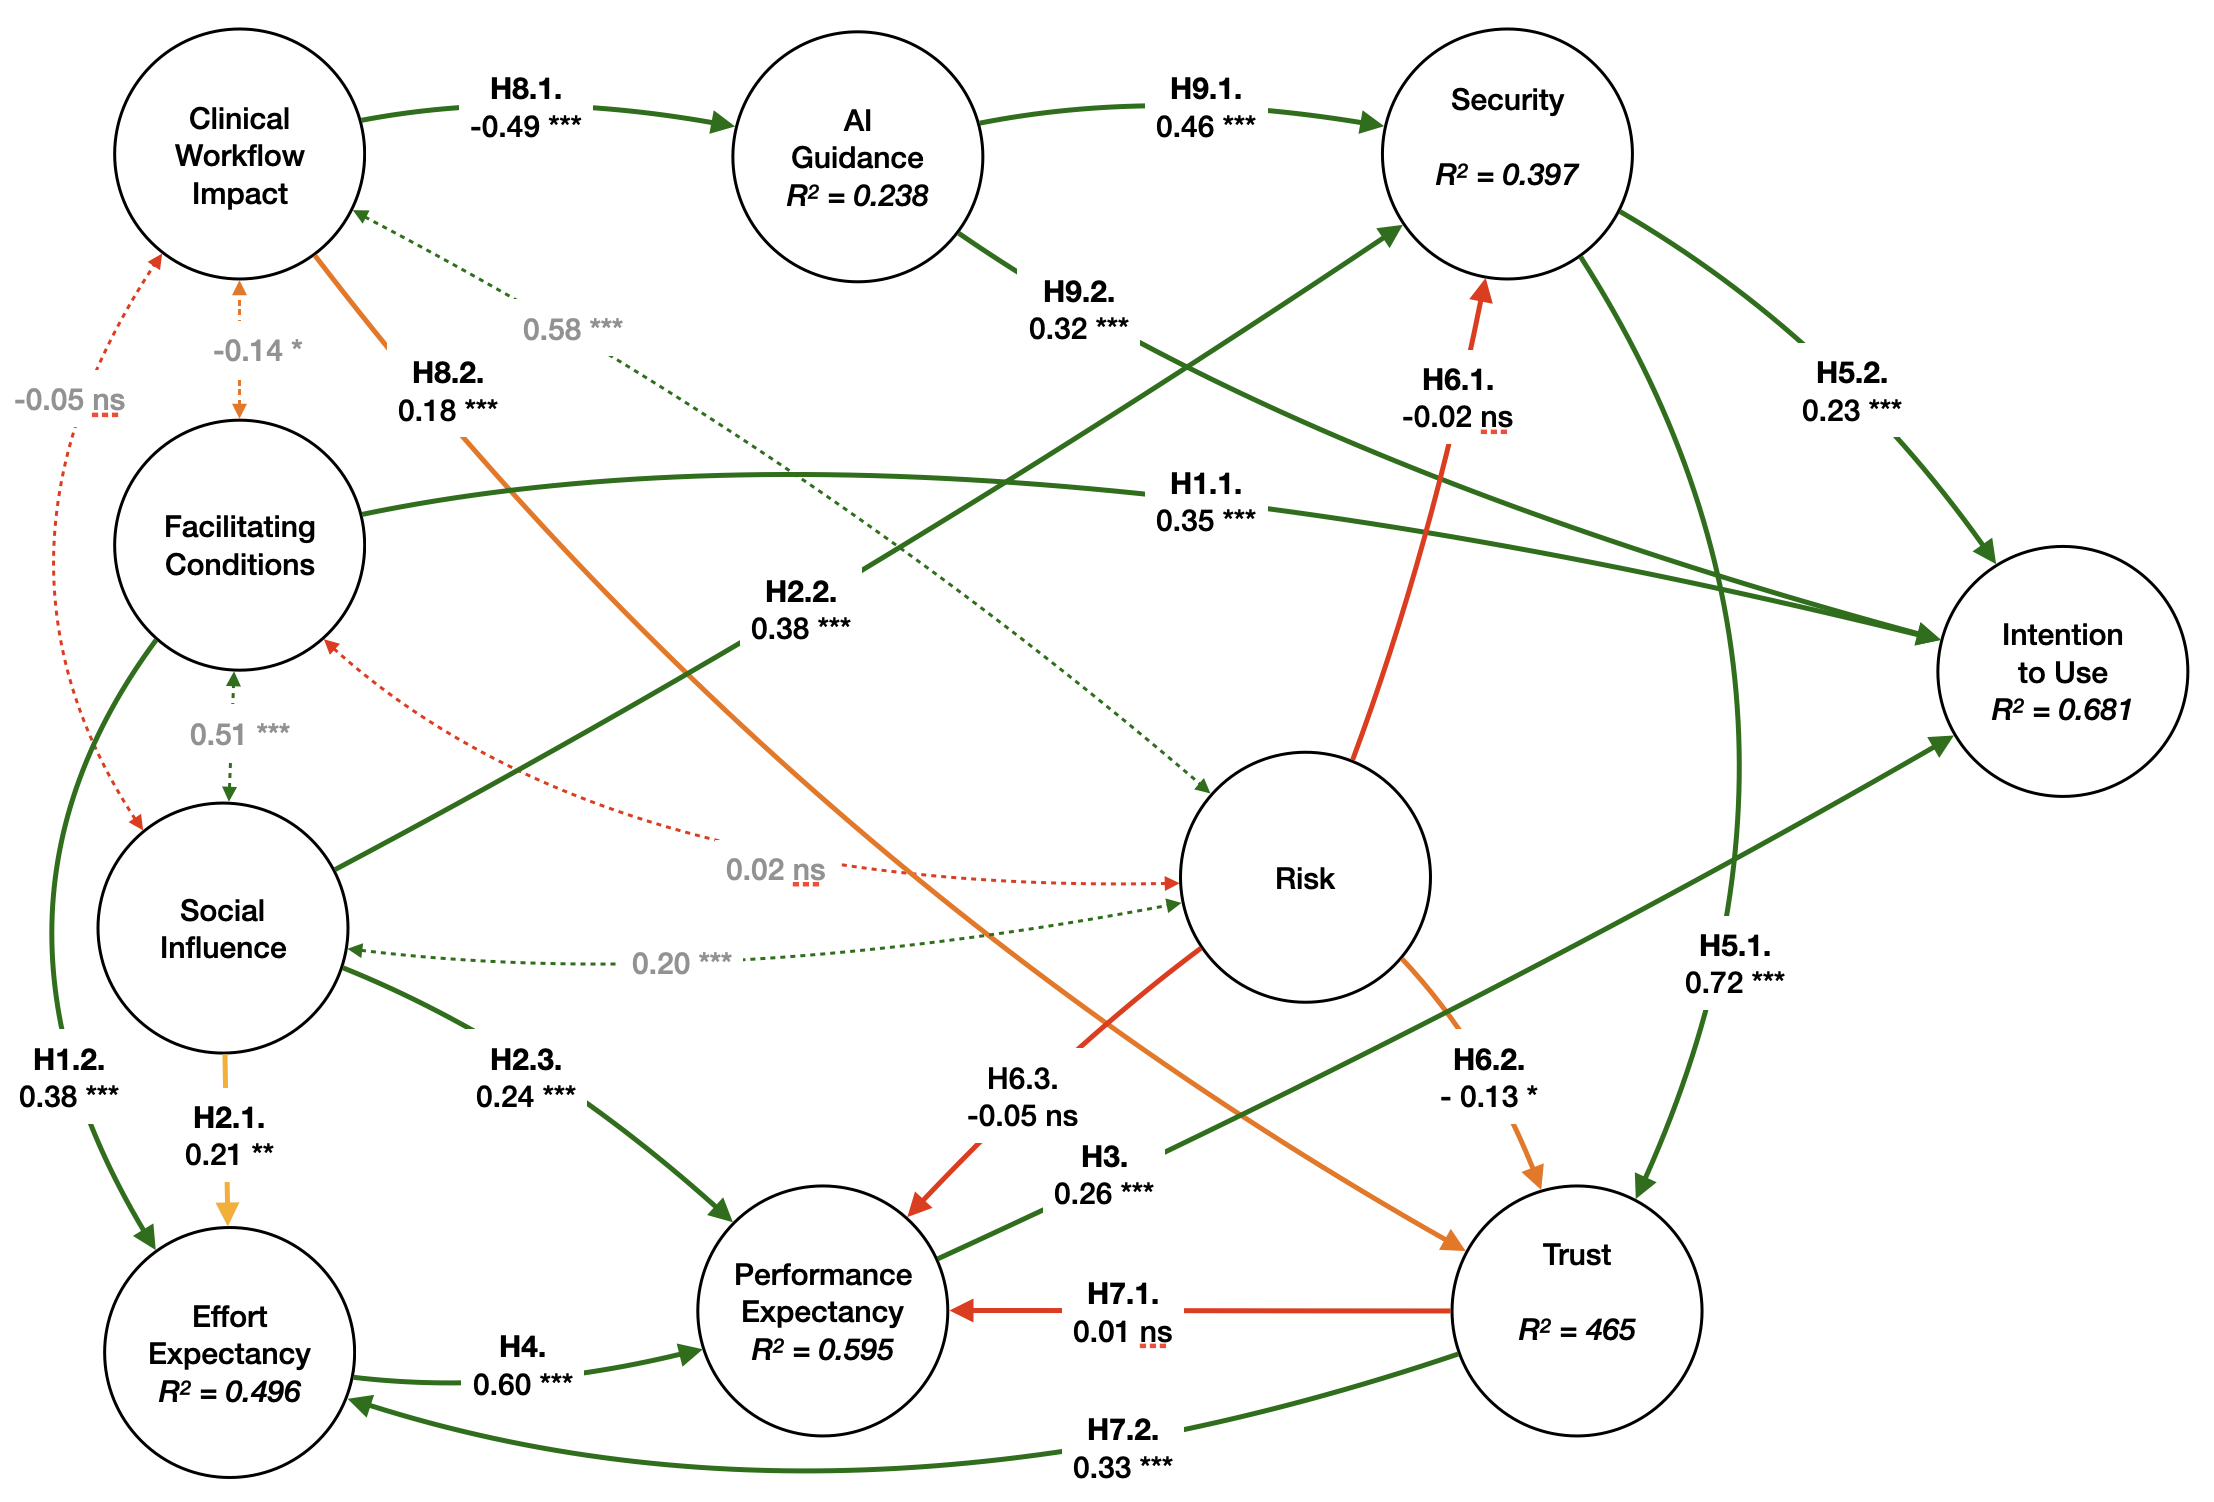
\includegraphics[width=0.985\linewidth]{fig074}
\caption{Detailed results of the research model. For beta results, the significance values are: in green for *** significant at level $\alpha = 0.01$; yellow for ** significant at $\alpha = 0.05$; orange for * significant fixed at $\alpha = 0.10$; and red for \underline{n}ot \underline{s}ignificant (ns).}
\label{fig:fig074}
\end{figure}
%%%%%%%%%%%%%%%%%%%%%%%%%%%%%%%%%%%%%%%%%%%%%%%%%%%

\textcolor{revised}{As detailed in Section~\ref{sec:chap004006002}, the design recommendations emerged from an iterative process of analyzing the empirical data in conjunction with the theoretical insights gained from our model.
Specifically, we scrutinized how clinicians' perceptions of security, risk, and trust influence their receptiveness to \ac{AI} recommendations.
This analysis was further enriched by integrating established concepts from the literature on \ac{AI} trustworthiness, bias mitigation, and the importance of explainable \ac{AI} in clinical settings.
Doing so ensured our recommendations are empirically grounded and theoretically robust, addressing critical concerns in deploying \ac{AI} in medical diagnostics.
The subsequent sections will elaborate on these recommendations, highlighting their practical implications for designing user-centric \ac{AI} tools in healthcare and how they contribute to the broader discourse on \ac{AI} adoption in clinical environments.}

\subsection{Main Findings}
\label{sec:chap004006001}

\textcolor{revised}{This section explores vital findings across factors like facilitating conditions and trust dynamics, illuminating the intricacies of clinician-\ac{AI} interactions and informing our design strategy.
Our exploration covers facilitating conditions (Section~\ref{sec:chap004006001001}), social influence (Section~\ref{sec:chap004006001002}), performance expectations (Section~\ref{sec:chap004006001003}), security (Section~\ref{sec:chap004006001004}), risk (Section~\ref{sec:chap004006001005}), trust (Section~\ref{sec:chap004006001006}), \ac{AI} guidance (Section~\ref{sec:chap004006001007}), and other factors (Section~\ref{sec:chap004006001008}), informing clinician perceptions and interactions with \ac{AI} systems.
This analysis highlights the need for a design framework that aligns with clinicians' ethos and needs, ensuring \ac{AI} tools are effective and meet their requirements.}

\subsubsection{Facilitating Factors}
\label{sec:chap004006001001}

\textcolor{revised}{Figure~\ref{fig:fig074} illustrates the key findings of our study, which significantly inform the design recommendations in Section~\ref{sec:chap004006002}.
Our analysis revealed that facilitating conditions are a strong predictor of clinicians' intention to use \ac{AI} in clinical workflows ({\bf H1.1.}), underscoring the importance of supportive environments for \ac{AI} adoption.
This finding aligns with existing literature emphasizing the role of facilitating conditions in enhancing user acceptance~\cite{Lambert2023, KHANIJAHANI2022100602}, particularly in these high-stakes domains.
Furthermore, our results demonstrate a notable link between facilitating conditions and effort expectancy ({\bf H1.2.}), suggesting that ease of use is a critical factor in clinician engagement with \ac{AI} tools.}

\subsubsection{Social Factors}
\label{sec:chap004006001002}

\textcolor{revised}{The influence of social factors was also evident, with social influence directly impacting effort expectancy ({\bf H2.1.}), perceived security ({\bf H2.2.}), and performance expectancy ({\bf H2.3.}).
This highlights the role of social dynamics when adopting \ac{AI} systems in healthcare settings.
These insights are grounded in the broader discourse on trust and bias in \ac{AI}~\cite{CHOUDHURY2022103708}, as social influence can shape clinicians' trust in \ac{AI} systems and potentially introduce biases in their adoption and use.}

\subsubsection{Performance Factors}
\label{sec:chap004006001003}

\textcolor{revised}{The study's findings underscore the significant role of performance expectancy in shaping clinicians' intention to use \ac{AI}, as evidenced by our hypothesis ({\bf H3.}), with a notable impact observed among {\it male expert} clinicians (Table~\ref{tab:tab012}).
This insight aligns with existing literature that emphasizes the importance of perceived effectiveness in technology adoption~\cite{SOLAIMANI2023101760, HSIEH2023107868}, particularly in complex clinical settings like medical imaging.
Effort expectancy's positive influence on performance expectancy ({\bf H4.}) further highlights the need for user-friendly \ac{AI} systems that can seamlessly integrate into clinical workflows, reducing the cognitive load on clinicians.}

\subsubsection{Security Factors}
\label{sec:chap004006001004}

\textcolor{revised}{Our analysis also reveals that security is a critical factor in building clinicians' trust in \ac{AI} systems ({\bf H5.1.}), influencing their attitudes and behavioral intentions ({\bf H5.2.}).
This finding is particularly relevant in healthcare, where data security and patient privacy are paramount~\cite{6038874, HLAVKA2020235}.
It suggests that design recommendations for \ac{AI} systems in medical imaging should prioritize robust security measures to foster trust among clinicians.
Furthermore, advanced security protocols protect sensitive data and boost clinicians' confidence in \ac{AI} tools~\cite{KHANIJAHANI2022100602}, promoting their acceptance and integration into clinical practice.}

\subsubsection{Risk Factors}
\label{sec:chap004006001005}

\textcolor{revised}{Additionally, perceived risk, as indicated by our hypothesis ({\bf H6.3.}), plays a pivotal role for certain clinician groups, affecting their beliefs about \ac{AI}'s performance and trust in maintaining patient privacy.
This observation is crucial for understanding the nuances of \ac{AI} adoption across different user demographics and specialties.
It points to the necessity of tailoring \ac{AI} systems to address specific concerns and biases~\cite{Topol2019, 10.1145/3290605.3300831}, ensuring that they are technically proficient and aligned with the medical field's ethical standards and privacy needs.}

\subsubsection{Trust Factors}
\label{sec:chap004006001006}

\textcolor{revised}{Our study reveals differences in trust's impact on performance expectancy ({\bf H7.1.}) and effort expectancy ({\bf H7.2.}) between {\it novice} and {\it expert} clinicians.
This highlights the need for adaptable \ac{AI} systems in healthcare, suitable for varying levels of clinician experience and trust.
Referencing the literature~\cite{gunning2017explainable, 10.1145/3411764.3445717}, we advocate for \ac{AI} systems with scalable guidance, particularly aiding novice clinicians.
These findings inform our design recommendations for personalized, context-specific \ac{AI} assistance.
Integrating \ac{XAI} principles~\cite{10.1145/2939672.2939778}, we aim to enhance transparency and reduce biases towards personalized \ac{AI} suggestions, building trust among clinicians with diverse expertise.
Therefore, adaptable and customized \ac{AI} guidance are essential characteristics for their effective adoption in various clinical settings.}

\subsubsection{Guidance Factors}
\label{sec:chap004006001007}

\textcolor{revised}{The impact of \ac{AI} guidance on security perceptions ({\bf H9.1.}) and behavioral intention ({\bf H9.2.}) varies among clinician groups, aligning with research highlighting security's importance in \ac{AI} systems~\cite{MALAMATENIOU20211192}.
Our design recommendations focus on integrating robust, adaptable security settings in diverse healthcare environments, essential for building trust and acceptance among various user demographics.
This approach, supported by literature on security's role in user trust~\cite{Amann2020}, also aligns with bias mitigation and system explainability efforts~\cite{SHIN2021102551}.
Recognizing these findings' variability, we emphasize the need for context-aware \ac{AI} solutions across different medical institutions, radiologists, and countries.}

\subsubsection{Other Factors}
\label{sec:chap004006001008}

\textcolor{revised}{While several hypotheses ({\it e.g.}, {\bf H6.1.}, {\bf H6.2.}, {\bf H8.1.}, or {\bf H8.2.}) did not find empirical support, our detailed examination in Section~\ref{chap:app002005001} of Appendix~\ref{chap:app002} delves deeper into these constructs.
This further analysis uncovers their relevance in particular contexts and for specific clinician groups, underscoring the necessity to cater to varied user needs and perceptions in \ac{AI} system design.
The findings inform our design recommendations, which emphasize the creation of \ac{AI} tools that are not just technically adept, but also resonate with the diverse expectations and requirements of different clinician demographics.}

\textcolor{revised}{The design recommendations in Section~\ref{sec:chap004006002} stem from analyzing empirical data and \ac{UTAUT}-based theoretical insights, focusing on clinicians' perceptions of security, risk, and trust in \ac{AI}.
Integrating literature on \ac{AI} trustworthiness~\cite{10.1145/3411764.3445717}, bias mitigation~\cite{10.1145/3290605.3300831}, and explainability~\cite{10.1145/2939672.2939778}, our recommendations are empirically and theoretically informed.
They emphasize enhancing facilitating conditions like comprehensive training to improve clinicians' effort expectancy and security perception.
Emphasizing transparency and explainability in \ac{AI} systems addresses biases and builds trust, aligning technology with clinical practice.
Grounded in empirical evidence and literature~\cite{CHOUDHURY2022103708}, we aim to develop effective, trustworthy \ac{AI} tools tailored to clinicians' diverse needs in medical imaging diagnosis.}

\subsection{Design Recommendations}
\label{sec:chap004006002}

\textcolor{revised}{Based on insights from Section~\ref{sec:chap004006001}, this section provides guidelines for integrating intelligent agents into medical imaging workflows, enhancing \ac{AI} as a supportive second-reader.
Trust, a crucial element for clinician engagement highlighted in literature~\cite{LIU2022107026}, is a vital focus of these guidelines.
Rooted in \ac{HCI} principles such as transparency, explainability, and workflow compatibility, the aim is to improve diagnostics and foster a synergistic clinician-\acs{AI} relationship.
Following a human-centered design approach~\cite{10.1145/3313831.3376718}, as we describe next in Chapter~\ref{chap:chap005}, these design recommendations strive to minimize cognitive load and enhance the \ac{UX} of clinicians during the interaction with intelligent agents, making \ac{AI} assistants more intuitive and user-friendly.}

\textcolor{revised}{Incorporating \ac{HCI} principles~\cite{Knisely2021}, the design recommendations advocate for adaptability, personalization, and cognitive load management in \ac{AI} systems, catering to the unique demands of clinical environments.
Usability and interpretability are pivotal for seamlessly integrating \ac{AI} tools into healthcare routines~\cite{10.1145/3411764.3445385}.
These principles ensure that \ac{AI} solutions are intuitive, reducing unnecessary cognitive burden and fostering an environment where clinicians and \ac{AI} systems work in tandem.
For a comprehensive overview of these design considerations, consult Section~\ref{chap:app002005002} in Appendix~\ref{chap:app002}.}

\vspace{1.50mm}

\noindent
\textcolor{revised}{Our design recommendations, grounded in empirical data and theoretical insights, include:}

\vspace{0.50mm}

\begin{enumerate}
\item \textcolor{revised}{Intelligent agents should clearly communicate the implications of \ac{AI} guidance on clinical workflow~\cite{MALAMATENIOU20211192}, offering clinicians control over decisions;}
\item \textcolor{revised}{An \ac{AI} systems must adapt communication to clinicians' demographic characteristics~\cite{Alowais2023}, including gender, age, and country development categories, to ensure effective and personalized interaction;}
\item \textcolor{revised}{An \ac{AI} systems should account for the variability in medical cases~\cite{10.1145/3313831.3376506}, tailoring their approach to individual conditions and diverse \ac{AI} techniques;}
\item \textcolor{revised}{Designers and developers should enhance the ease of use (usability) and usefulness (functionality) of \ac{AI} systems to improve perceived security, perceived risk, and trust of clinicians~\cite{OPRESCU202253}.}
\end{enumerate}

\textcolor{revised}{These recommendations, informed by our study, focus on providing informative \ac{AI} guidance, personalizing communication, considering case variability, and enhancing usability and functionality.
They are designed to facilitate the effective integration of \ac{AI} technology in medical imaging's clinical workflow.
Additionally, they aim to bridge the gap between technological capabilities and clinical needs, ensuring that \ac{AI} tools are advanced and intuitively align with clinicians' daily practices.
The recommendations seek to improve diagnostic accuracy and efficiency by addressing these critical areas, ultimately improving patient outcomes.
For more detailed design considerations, please see Section~\ref{chap:app002005002} of Appendix~\ref{chap:app002}.}

\section{Boundaries}
\label{sec:chap004007}

Despite its contributions, the study has some boundaries, which provide fruitful avenues for further research.
Several of these boundaries affect the scope of our results.
Although we had a significant sample of global nationalities, there is still a bias for the small sample size (Table~\ref{tab:tab008}) of specific nationalities.
To understand the effect of this bias, we analyzed the moderator effect of country development categories in our model, which showed the same evidence of invariant measure compared to other moderators (gender, age, etc.).
However, we did not record race and ethnicity differences in our sample.
Previous works show a significant impact of cultural diversity on social influence, usefulness, and behavior intention~\cite{Belanche2019, info:doi/10.2196/27122}.

Another limitation of our study is that it involved clinicians mainly related to radiology.
Given the focus of our study, {\it i.e.}, the medical imaging field, our sample could be biased.
The effect of such characteristics limits the generalizability of this research, since the sample employed in this study could express different perceptions towards \ac{AI} systems compared to other clinical expertise.
However, the experimental design helps reduce the impact of the \ac{CMB}, which we employed in this study, particularly for the new \ac{AI} constructs.
Moreover, by combining the survey with outcome variables measured separately and more objectively ({\it e.g.}, frequency of usage/reporting), we are revealing valid results less prone to measurement and method bias.

Despite the above boundaries, this study fosters the community's understanding of the intention to use \ac{AI} systems in the clinical workflow. Specifically for the associated constructs of security, risk, and trust concerns on \ac{AI} systems.
Finally, we provide valuable design guidelines and recommendations for delivering \ac{AI} systems with these concerns to different user groups.

\section{Conclusion}
\label{sec:chap004008}

In this chapter, we conducted a comprehensive investigation into the acceptance and adoption of \ac{AI} systems in the clinical workflow of medical imaging diagnosis.
The study focused on understanding the role of security, risk, and trust in influencing clinicians' acceptance of \ac{AI}-based assistance.
Through empirical testing, we confirmed that trust plays a critical role in shaping user acceptance, mediating the effects of \ac{AI}-specific aspects of user behavior.
Additionally, clinicians' demographic characteristics, such as gender, age, and educational background, moderate the relationship between these factors and their intention to use \ac{AI} systems.
These findings underscore the importance of considering clinicians' specific needs and characteristics when developing intelligent agents for medical imaging diagnosis.
Integrating \ac{HCI} principles into developing \ac{AI}-based assistance to create user-friendly and effective systems, enhancing clinical workflows and improving patient outcomes.

The research conducted in this chapter provides valuable insights and implications for the design, development, and deployment of \ac{AI}-based assistance in healthcare.
The study highlights the significance of trust, addresses security, and risk concerns, while offering practical guidelines for integrating \ac{AI} systems into the clinical workflow, building upon the design interventions discussed in Chapter~\ref{chap:chap005}.
Chapter~\ref{chap:chap006} further explores the importance of tailoring communication methods to address the specific needs of different user groups, enhancing clinicians' engagement and acceptance of \ac{AI} technology.
This comprehensive approach, encompassing adoption studies (Chapter~\ref{chap:chap004}), design interventions (Chapter~\ref{chap:chap005}), and tailored adaptive communication (Chapter~\ref{chap:chap006}), promotes the successful acceptance and integration of \ac{AI} systems in healthcare settings.
The final remarks can be found in Section~\ref{chap:app002006} of Appendix~\ref{chap:app002}, providing a more comprehensive and in-depth perspective on the summarized conclusions.